% memorder/memorder.tex

\QuickQuizChapter{chp:memorder:Memory Ordering}{Memory Ordering}
\OriginallyPublished{Chapter}{chp:memorder:Memory Ordering}{Linux Kernel Memory Barriers}{kernel.org}{Howells2009membartxt}
\OriginallyPublished{Chapter}{chp:memorder:Memory Ordering}{A formal kernel memory-ordering model}{Linux Weekly News}{JadeAlglave2017LWN-LKMM-1,JadeAlglave2017LWN-LKMM-2}
%
\Epigraph{The art of progress is to preserve order amid change and to preserve change amid order.}{\emph{Alfred North Whitehead}}

Causality and sequencing are deeply intuitive, and hackers often
tend to have a much stronger grasp of these concepts than does
the general population.
These intuitions can be extremely powerful tools when writing, analyzing,
and debugging both sequential code and parallel code that makes
use of standard mutual-exclusion mechanisms, such as locking and
RCU.
Unfortunately, these intuitions break down completely in face of
code that fails to use standard mechanisms, one important example
of course being the code that implements these standard mechanisms.
This chapter will help you gain an understanding of memory ordering
sufficient to implement synchronization primitives and other
performance-critical code.

@@@ roadmap @@@

\section{Ordering: Why and How?}
\label{sec:memorder:Ordering: Why and How?}

One motivation for memory ordering can be seen in the trivial-seeming
litmus test in
Listing~\ref{lst:memorder:Memory Misordering: Store-Buffering Litmus Test}
(\path{C-SB+o-o+o-o.litmus}),
which at first glance might
appear to guarantee that the \co{exists} clause never triggers.\footnote{
	Purists would instead say that the \co{exists} clause is
	never \emph{satisfied}, but we use ``trigger'' here by
	analogy with assertions.}
After all, if \nbco{0:r2=0} as shown in the \co{exists} clause,\footnote{
	That is, Thread~\co{P0()}'s instance of local variable \co{r2}
	equals zero.
	See Section~\ref{sec:formal:Anatomy of a Litmus Test}
	for documentation of litmus-test nomenclature.}
we might hope that Thread~\co{P0()}'s
load from~\co{x1} must have happened before Thread~\co{P1()}'s store to~\co{x1},
which might raise
further hopes that Thread~\co{P1()}'s load from~\co{x0} must happen after
Thread~\co{P0()}'s store to~\co{x0}, so that \nbco{1:r2=2},
thus not triggering the \co{exists} clause.
The example is symmetric, so similar reasoning might lead
us to hope that \nbco{1:r2=0} guarantees that \nbco{0:r2=2}.
Unfortunately, the lack of memory barriers dashes these hopes.
The CPU is within its rights to reorder
the statements within both Thread~\co{P0()} and Thread~\co{P1()},
even on relatively strongly ordered systems such as x86.

\begin{listing}[tbp]
{ \scriptsize
\begin{verbbox}[\LstLineNo]
C C-SB+o-o+o-o
{
}

P0(int *x0, int *x1)
{
  int r2;

  WRITE_ONCE(*x0, 2);
  r2 = READ_ONCE(*x1);
}


P1(int *x0, int *x1)
{
  int r2;

  WRITE_ONCE(*x1, 2);
  r2 = READ_ONCE(*x0);
}

exists (1:r2=0 /\ 0:r2=0)
\end{verbbox}
}
\centering
\theverbbox
\caption{Memory Misordering: Store-Buffering Litmus Test}
\label{lst:memorder:Memory Misordering: Store-Buffering Litmus Test}
\end{listing}

\QuickQuiz{}
	The compiler can also reorder Thread~\co{P0()}'s and
	Thread~\co{P1()}'s memory accesses in
	Listing~\ref{lst:memorder:Memory Misordering: Store-Buffering Litmus Test},
	right?
\QuickQuizAnswer{
	In general, compiler optimizations carry out more extensive
	and profound reorderings than CPUs can.
	However, in this case, the volatile accesses in
	\co{READ_ONCE()} and \co{WRITE_ONCE()}
	prevent the compiler from reordering.
	And also from doing much else as well, so the examples in this
	section will be making heavy use of
	\co{READ_ONCE()} and \co{WRITE_ONCE()}.
	% @@@ forward reference to a section describing READ_ONCE()
	% @@@ and WRITE_ONCE().
} \QuickQuizEnd

This willingness to reorder can be confirmed using tools such as
\co{litmus7}~\cite{Alglave:2014:HCM:2594291.2594347},
which found that the counter-intuitive ordering happened
314 times out of 100,000,000 trials on my x86 laptop.
Oddly enough, the perfectly legal outcome where both loads return the
value 2 occurred less frequently, in this case, only 167 times.\footnote{
	Please note that results are sensitive to the exact hardware
	configuration,
	how heavily the system is loaded, and much else besides.}
The lesson here is clear: Increased counterintuitivity does not necessarily
imply decreased probability!
% Run on June 23, 2017:
% litmus7 -r 1000 -carch X86 C-SB+o-o+o-o.litmus
% Test C-SB+o-o+o-o Allowed
% Histogram (4 states)
% 314   *>0:r2=0; 1:r2=0;
% 49999625:>0:r2=2; 1:r2=0;
% 49999894:>0:r2=0; 1:r2=2;
% 167   :>0:r2=2; 1:r2=2;

The following sections show exactly where this intuition breaks down,
and then puts forward a mental model of memory ordering that can help
you avoid these pitfalls.

Section~\ref{sec:memorder:Why Hardware Misordering?}
gives a brief overview of why hardware misorders memory accesses, and then
Section~\ref{sec:memorder:How to Force Ordering?}
gives an equally brief overview of how you can thwart evil hardware
misordering schemes.
Finally, Section~\ref{sec:memorder:Basic Rules of Thumb}
lists some basic rules of thum, which will be further refined in
later sections.

\subsection{Why Hardware Misordering?}
\label{sec:memorder:Why Hardware Misordering?}

But why does memory misordering happen in the first place?
Can't CPUs keep track of ordering on their own?
Isn't that why we have computers in the first place, to keep track of things?

Many people do indeed expect their computers to keep track of things,
but many also insist that they keep track of things quickly.
However, as seen in Chapter~\ref{chp:Hardware and its Habits},
one difficulty that modern computer-system vendors face is that
the main memory cannot keep up with the CPU---modern CPUs can execute
hundreds of instructions in the time required to fetch a single variable
from memory.
CPUs therefore sport increasingly large caches, as seen back in
Figure~\ref{fig:cpu:System Hardware Architecture}, which means that
although the first load by a given CPU from a given variable will
result in an expensive \emph{cache miss} as was discussed in
Section~\ref{sec:cpu:Cache Misses}, subsequent
repeated loads from that variable by that CPU might execute
very quickly because the initial cache miss will have loaded that
variable into that CPU's cache.

However, it is also necessary to accommodate frequent concurrent stores
from multiple CPUs to a set of shared variables.
In cache-coherent systems, if the caches hold multiple copies of a given
variable, all the copies of that variable must have the same value.
This works extremely well for concurrent loads, but not so well for
concurrent stores:  Each store must do something about all
copies of the old value (another cache miss!), which, given the finite
speed of light and the atomic nature of matter, will be slower
than impatient software hackers would like.

\begin{figure}[tb]
\centering
\resizebox{2.5in}{!}{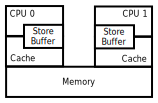
\includegraphics{memorder/SystemArchSB}}
\caption{System Architecture With Store Buffers}
\label{fig:memorder:System Architecture With Store Buffers}
\end{figure}

CPUs therefore come equipped with store buffers, as shown in
Figure~\ref{fig:memorder:System Architecture With Store Buffers}.
When a given CPU does a store to a variable that
is not present in that CPU's cache, then the new value
is instead placed in that CPU's store buffer.
The CPU can then proceed immediately, without having to wait for the
store to do something about all the old values of that variable
residing in other CPUs' caches.

\begin{figure}[htb]
\centering
\resizebox{3in}{!}{\includegraphics{cartoons/r-2014-Out-of-order}}
\caption{CPUs Can Do Things Out of Order}
\ContributedBy{Figure}{fig:memorder:CPUs Can Do Things Out of Order}{Melissa Broussard}
\end{figure}

Although store buffers can greatly increase performance,
they can cause instructions and memory references to execute out
of order, which can in turn cause serious confusion, as illustrated in
Figure~\ref{fig:memorder:CPUs Can Do Things Out of Order}.
In particular, these store buffers can cause the memory misordering
shown in the store-buffering litmus test in
Listing~\ref{lst:memorder:Memory Misordering: Store-Buffering Litmus Test}.

\begin{table*}
\small
\centering\OneColumnHSpace{-0.1in}
\begin{tabular}{r||l|l|l||l|l|l}
	& \multicolumn{3}{c||}{CPU 0} & \multicolumn{3}{c}{CPU 1} \\
	\cline{2-7}
	& Instruction & Store Buffer & Cache &
		Instruction & Store Buffer & Cache \\
	\hline
	\hline
	1 & (Initial state) & & \tco{x1==0} &
		(Initial state) & & \tco{x0==0} \\
	\hline
	2 & \tco{x0 = 2;} & \tco{x0==2} & \tco{x1==0} &
		\tco{x1 = 2;} & \tco{x1==2} & \tco{x0==0} \\
	\hline
	3 & \tco{r2 = x1;} (0) & \tco{x0==2} & \tco{x1==0} &
		\tco{r2 = x0;} (0) & \tco{x1==2} & \tco{x0==0} \\
	\hline
	4 & (Read-invalidate) & \tco{x0==2} & \tco{x0==0} &
		(Read-invalidate) & \tco{x1==2} & \tco{x1==0} \\
	\hline
	5 & (Finish store) & & \tco{x0==2} &
		(Finish store) & & \tco{x1==2} \\
\end{tabular}
\caption{Memory Misordering: Store-Buffering Sequence of Events}
\label{tab:memorder:Memory Misordering: Store-Buffering Sequence of Events}
\end{table*}

Table~\ref{tab:memorder:Memory Misordering: Store-Buffering Sequence of Events}
shows how this memory misordering can happen.
Row~1 shows the initial state, where CPU~0 has \co{x1} in its cache
and CPU~1 has \co{x0} in its cache, both variables having a value of zero.
Row~2 shows the state change due to each CPU's store (lines~9 and~18 of
Listing~\ref{lst:memorder:Memory Misordering: Store-Buffering Litmus Test}).
Because neither CPU has the stored-to variable in its cache, both CPUs
record their stores in their respective store buffers.

\QuickQuiz{}
	But wait!!!
	On row~2 of
	Table~\ref{tab:memorder:Memory Misordering: Store-Buffering Sequence of Events}
	both \co{x0} and \co{x1} each have two values at the same time,
	namely zero and two.
	How can that possibly work???
\QuickQuizAnswer{
	There is an underlying cache-coherence protocol that straightens
	things out, which will be discussed later.
	% @@@ Add forward reference.
	But if you think that a given variable having two values at
	the same time is surprising, just wait until you get to
	Section~\ref{sec:memorder:Variables With Multiple Values}!
} \QuickQuizEnd

Row~3 shows the two loads (lines~10 and~19 of
Listing~\ref{lst:memorder:Memory Misordering: Store-Buffering Litmus Test}).
Because the variable being loaded by each CPU is in that CPU's cache,
each load immediately returns the cached value, which in both cases
is zero.

But the CPUs are not done yet: Sooner or later, they must empty their
store buffers.
Because caches move data around in relatively large blocks called
\emph{cachelines}, and because each cacheline can hold several
variables, each CPU must get the cacheline into its own cache so
that it can update the portion of that cacheline corresponding
to the variable in its store buffer, but without disturbing any
other part of the cacheline.
Each CPU must also ensure that the cacheline is not present in any other
CPU's cache, for which a read-invalidate operation is used.
As shown on row~4, after both read-invalidate operations complete,
the two CPUs have traded cachelines, so that CPU~0's cache now contains
\co{x0} and CPU~1's cache now contains \co{x1}.
Once these two variables are in their new homes, each CPU can flush
its store buffer into the corresponding cache line, leaving each
variable with its final value as shown on row~5.

\QuickQuiz{}
	But don't the values also need to be flushed from the cache
	to main memory?
\QuickQuizAnswer{
	Perhaps surprisingly, not necessarily!
	On some systems,
	if the two variables are being used heavily, they might
	be bounced back and forth between the CPUs' caches and never
	land in main memory.
} \QuickQuizEnd

In summary, store buffers are needed to allow CPUs to handle
store instructions efficiently, but they can result in
counter-intuitive memory misordering.

But what do you do if your algorithm really needs its memory
references to be ordered?
For example, suppose that you are communicating with a driver using
a pair of flags, one that says whether or not the driver is running
and the other that says whether there is a request pending for that
driver.
The requester needs to set the request-pending flag, then check
the driver-running flag, and if false, wake it up.
Once the driver has serviced all the pending requests that it knows about,
it needs to clear its driver-running flag, then check the request-pending
flag to see if it needs to restart.
This very reasonable approach cannot work unless there is some way
to make sure that the hardware processes the stores and loads in order.
This is the subject of the next section.

\subsection{How to Force Ordering?}
\label{sec:memorder:How to Force Ordering?}

It turns out that there are compiler directives and standard
synchronization primitives (such as locking and RCU)
that are responsible for maintaining the illusion of ordering through use of
\emph{memory barriers} (for example, \co{smp_mb()} in the Linux kernel).
These memory barriers can be explicit instructions, as they are on
ARM, POWER, Itanium, and Alpha, or they can be implied by other instructions,
as they often are on x86.
Since these standard synchronization primitives preserve the illusion of
ordering, your path of least resistance is to simply use these primitives,
thus allowing you to stop reading this section.

\begin{listing}[tbp]
{ \scriptsize
\begin{verbbox}[\LstLineNo]
C C-SB+o-mb-o+o-mb-o
{
}

P0(int *x0, int *x1)
{
  int r2;

  WRITE_ONCE(*x0, 2);
  smp_mb();
  r2 = READ_ONCE(*x1);
}


P1(int *x0, int *x1)
{
  int r2;

  WRITE_ONCE(*x1, 2);
  smp_mb();
  r2 = READ_ONCE(*x0);
}

exists (1:r2=0 /\ 0:r2=0)
\end{verbbox}
}
\centering
\theverbbox
\caption{Memory Ordering: Store-Buffering Litmus Test}
\label{lst:memorder:Memory Ordering: Store-Buffering Litmus Test}
\end{listing}

However, if you need to implement the synchronization primitives
themselves, or if you are simply interested in understanding how memory
ordering works, read on!
The first stop on the journey is
Listing~\ref{lst:memorder:Memory Ordering: Store-Buffering Litmus Test}
(\path{C-SB+o-mb-o+o-mb-o.litmus}),
which places an \co{smp_mb()} Linux-kernel full memory barrier between
the store and load in both \co{P0()} and \co{P1()}, but is otherwise
identical to
Listing~\ref{lst:memorder:Memory Misordering: Store-Buffering Litmus Test}.
% Test C-SB+o-mb-o+o-mb-o Allowed
% Histogram (3 states)
% 49553298:>0:r2=2; 1:r2=0;
% 49636449:>0:r2=0; 1:r2=2;
% 810253:>0:r2=2; 1:r2=2;
% No
These barriers prevent the counter-intuitive outcome from happening
on 100,000,000 trials on my x86 laptop.
Interestingly enough, the added overhead due to these barriers causes the
legal outcome where both loads return the value two to happen more
than 800,000 times, as opposed to only 167 times for the
barrier-free code in
Listing~\ref{lst:memorder:Memory Misordering: Store-Buffering Litmus Test}.

\begin{table*}
\small
\centering\OneColumnHSpace{-0.1in}
\begin{tabular}{r||l|l|l||l|l|l}
	& \multicolumn{3}{c||}{CPU 0} & \multicolumn{3}{c}{CPU 1} \\
	\cline{2-7}
	& Instruction & Store Buffer & Cache &
		Instruction & Store Buffer & Cache \\
	\hline
	\hline
	1 & (Initial state) & & \tco{x1==0} &
		(Initial state) & & \tco{x0==0} \\
	\hline
	2 & \tco{x0 = 2;} & \tco{x0==2} & \tco{x1==0} &
		\tco{x1 = 2;} & \tco{x1==2} & \tco{x0==0} \\
	\hline
	3 & \tco{smp_mb();} & \tco{x0==2} & \tco{x1==0} &
		\tco{smp_mb();} & \tco{x1==2} & \tco{x0==0} \\
	\hline
	4 & (Read-invalidate) & \tco{x0==2} & \tco{x0==0} &
		(Read-invalidate) & \tco{x1==2} & \tco{x1==0} \\
	\hline
	5 & (Finish store) & & \tco{x0==2} &
		(Finish store) & & \tco{x1==2} \\
	\hline
	6 & \tco{r2 = x1;} (2) & & \tco{x1==2} &
		\tco{r2 = x0;} (2) & & \tco{x0==2} \\
\end{tabular}
\caption{Memory Ordering: Store-Buffering Sequence of Events}
\label{tab:memorder:Memory Ordering: Store-Buffering Sequence of Events}
\end{table*}

These barriers have a profound effect on ordering, as can be seen in
Table~\ref{tab:memorder:Memory Ordering: Store-Buffering Sequence of Events}.
Although the first two rows are the same as in
Table~\ref{tab:memorder:Memory Misordering: Store-Buffering Sequence of Events}
and although the \co{smp_mb()} instructions on row~3
do not change state
in and of themselves, they do cause the stores to complete
(rows~4 and~5) before the
loads (row~6), which rules out the counter-intuitive outcome shown in
Table~\ref{tab:memorder:Memory Misordering: Store-Buffering Sequence of Events}.
Note that variables \co{x0} and \co{x1} each still have more than one
value on row~2, however, as promised earlier, the \co{smp_mb()}
instances straighten things out in the end.

\begin{table*}
\small
\centering\OneColumnHSpace{-0.7in}
\begin{tabular}{l||c||c|c|c|c||c|c|c|c|c|c|c}
	& & \multicolumn{4}{c||}{Prior Ordered Operation} &
		\multicolumn{7}{c}{Subsequent Ordered Operation} \\
	\cline{3-6} \cline{7-13}
	Operation Providing Ordering & C &
		Self & R & W & RMW & Self & R & W & DR & DW & RMW & SV \\
	\hline
	\hline
	Store, for example, \tco{WRITE_ONCE()} &  &
		   Y &   &   &     &      &   &   &    &    &     &  Y \\
	\hline
	Load, for example, \tco{READ_ONCE()} &  &
		   Y &   &   &     &      &   &   &    &  Y &     &  Y \\
	\hline
	Unsuccessful RMW operation &  &
		   Y &   &   &     &      &   &   &    &  Y &     &  Y \\
	\hline
	\tco{smp_read_barrier_depends()} &  &
		     & Y &   &     &      &   &   &  Y &  Y &     &    \\
	\hline
	\tco{*_dereference()} &  &
		   Y &   &   &     &      &   &   &  Y &  Y &     &  Y \\
	\hline
	Successful \tco{*_acquire()} &   &
		   R &   &   &     &      & Y & Y &  Y &  Y &   Y &  Y \\
	\hline
	Successful \tco{*_release()} & C &
		     & Y & Y &   Y &    W &   &   &    &    &     &  Y \\
	\hline
	\tco{smp_rmb()} &   &
		     & Y &   &   R &      & Y &   &  Y &    &   R &    \\
	\hline
	\tco{smp_wmb()} &   &
		     &   & Y &   W &      &   & Y &    &  Y &   W &    \\
	\hline
	\tco{smp_mb()} & CP &
		     & Y & Y &   Y &      & Y & Y &  Y &  Y &   Y &    \\
	\hline
	Successful full-strength non-\tco{void} RMW & CP &
		   Y & Y & Y &   Y &    Y & Y & Y &  Y &  Y &   Y &  Y \\
	\hline
	\tco{smp_mb__before_atomic()} & CP &
		     & Y & Y &   Y &      & a & a & a  & a  &   Y &    \\
	\hline
	\tco{smp_mb__after_atomic()} & CP &
		     & a & a &   Y &      & Y & Y &  Y &  Y &     &    \\
	\multicolumn{13}{c}{~} \\
	\multicolumn{1}{r}{Key:} &
		\multicolumn{12}{l}{C: Ordering is cumulative} \\
	\multicolumn{1}{r}{} &
		\multicolumn{12}{l}{P: Ordering propagates} \\
	\multicolumn{1}{r}{} &
		\multicolumn{12}{l}{R: Read, for example, \tco{READ_ONCE()}, or read portion of RMW} \\
	\multicolumn{1}{r}{} &
		\multicolumn{12}{l}{W: Write, for example, \tco{WRITE_ONCE()}, or write portion of RMW} \\
	\multicolumn{1}{r}{} &
		\multicolumn{12}{l}{Y: Provides the specified ordering} \\
	\multicolumn{1}{r}{} &
		\multicolumn{12}{l}{a: Provides specified ordering given intervening RMW atomic operation} \\
	\multicolumn{1}{r}{} &
		\multicolumn{12}{l}{DR: Dependent read (address dependency, Section~\ref{sec:memorder:Address Dependencies})} \\
	\multicolumn{1}{r}{} &
		\multicolumn{12}{l}{DW: Dependent write (address, data, or control dependency, Sections~\ref{sec:memorder:Address Dependencies}--\ref{sec:memorder:Control Dependencies})} \\
	\multicolumn{1}{r}{} &
		\multicolumn{12}{l}{RMW: Atomic read-modify-write operation} \\
	\multicolumn{1}{r}{} &
		\multicolumn{12}{l}{SV: Same-variable access} \\
\end{tabular}
\caption{Linux-Kernel Memory-Ordering Cheat Sheet}
\label{tab:memorder:Linux-Kernel Memory-Ordering Cheat Sheet}
\end{table*}

Although \co{smp_mb()} has extremely strong ordering guarantees, its strength
comes at a high price.
A great many situations can be handled with much weaker ordering guarantees
that use much cheaper memory-ordering instructions, or, in some case, no
memory-ordering instructions at all.
Table~\ref{tab:memorder:Linux-Kernel Memory-Ordering Cheat Sheet}
provides a cheatsheet of the Linux kernel's ordering primitives and their
guarantees.
Each row corresponds to a primitive or category of primitives that might
or might not provide ordering, with the columns labeled
``Prior Ordered Operation'' and ``Subsequent Ordered Operation''
being the operations that might (or might not) be ordered against.
Cells containing ``Y'' indicate that ordering is supplied unconditionally,
while other characters indicate that ordering is supplied only partially or
conditionally.
Blank cells indicate that no ordering is supplied.

The \co{*_acquire} row covers \co{smp_load_acquire()},
\co{cmpxchg_acquire()}, \co{xchg_acquire()}, and so on;
the \co{*_release} row covers \co{smp_store_release()},
\co{cmpxchg_release()}, \co{xchg_release()}, and so on; and
the ``Successful full-strength non-\co{void} RMW'' row covers
\co{atomic_add_return()}, \co{atomic_add_unless()}, \co{atomic_dec_and_test()},
\co{cmpxchg()}, \co{xchg()}, and so on.
The ``Successful'' qualifiers apply to primitives such as
\co{atomic_add_unless()}, \co{cmpxchg_acquire()}, and \co{cmpxchg_release()},
which have no effect on either memory or on ordering when they indicate
failure, as indicated by the earlier ``Unsuccessful RMW operation'' row.

Column ``C'' indicates cumulativity and propagation, as explained in
Sections~\ref{sec:memorder:Cumulativity}
and~\ref{sec:memorder:Propagation}.
In the meantime, this column can usually be ignored when there
are at most two threads involved.

\QuickQuiz{}
	The rows in
	Table~\ref{tab:memorder:Linux-Kernel Memory-Ordering Cheat Sheet}
	seem quite random and confused.
	Whatever is the conceptual basis of this table???
\QuickQuizAnswer{
	The rows correspond roughly to hardware mechanisms of increasing
	power and overhead.

	The \co{WRITE_ONCE()} row captures the fact that accesses to
	a single variable are always fully ordered, as indicated by
	the ``SV''column.
	Note that all other operations providing ordering against an
	access to a
	specific variable also provide this same-variable ordering.

	The \co{READ_ONCE()} row captures the fact that (as of 2017) compilers
	and CPUs do not indulge in user-visible speculative stores, so that
	any store whose address, data, or execution depends on a prior load
	will happen after that load completes.
	At least assuming that these dependencies have been constructed
	carefully as described in
	Sections~\ref{sec:memorder:Address- and Data-Dependency Restrictions}
	and~\ref{sec:memorder:Control-Dependency Restrictions}.

	The ``Unsuccessful RMW operation'' row captures the fact that
	even an unsuccessful RMW has done a read, and that read is
	every bit as good as a \co{READ_ONCE()}.

	The \co{smp_read_barrier_depends()} row captures the fact that, with the
	notable exception of DEC Alpha, compilers and CPUs do not indulge
	in user-visible breakage of address dependencies, again assuming
	that these dependencies have been constructed carefully as described in
	Section~\ref{sec:memorder:Address- and Data-Dependency Restrictions}.

	The \co{*_dereference()} row captures the address and data
	dependency ordering provided by \co{lockless_dereference()},
	\co{rcu_dereference()}, and friends.

	The ``Successful \co{*_acquire()}'' row captures the fact that many
	CPUs have special ``acquire'' forms of loads and of atomic RMW
	instructions,
	and that many other CPUs have light-weight memory-barrier
	instructions that order prior loads against subsequent loads
	and stores.

	The ``Successful \co{*_release()}'' row captures the fact that many
	CPUs have special ``release'' forms of stores and of atomic RMW
	instructions, and that many other CPUs have light-weight memory-barrier
	instructions that order prior loads and stores against
	subsequent stores.

	The \co{smp_rmb()} row captures the fact that many CPUs have
	light-weight memory-barrier instructions that order prior loads against
	subsequent loads.
	Similarly,
	the \co{smp_wmb()} row captures the fact that many CPUs have
	light-weight memory-barrier instructions that order prior stores against
	subsequent stores.

	None of the ordering operations thus far require prior stores to be
	ordered against subsequent loads, which means that these operations
	need not interfere with store buffers, whose main purpose in life
	is in fact to reorder prior stores against subsequent loads.
	The light-weight nature of these operations is precisely due to
	their policy of store-buffer non-interference.
	However, as noted earlier, it is sometimes necessary to interfere
	with the store buffer in order to prevent prior stores from being
	reordered against later stores, which brings us to the remaining
	rows in this table.

	The \co{smp_mb())} row corresponds to the full memory barrier
	available on most platforms, with Itanium being the exception
	that proves the rule.

	The ``Successful full-strength non-\co{void} RMW'' row captures
	the fact that on some platforms (such as x86) atomic RMW instructions
	provide full ordering both before and after.
	The Linux kernel therefore requires that full-strength non-\co{void}
	atomic RMW operations provide full ordering in cases where these
	operations succeed.
	(Full-strength atomic RMW operation's names do not end in
	\co{_relaxed}, \co{_acquire}, or \co{_release}.)

	However, the Linux kernel does not require that \co{void} atomic
	RMW operations provide any ordering whatsoever, with the
	canonical example being \co{atomic_inc()}.
	Therefore, these operations, along with failing non-\co{void}
	atomic RMW operations may be preceded by \co{smp_mb__before_atomic()}
	and followed by \co{smp_mb__after_atomic()} to provide full
	ordering for any accesses preceding or following both.
	No ordering need be provided for accesses between the
	\co{smp_mb__before_atomic()} (or, similarly, the
	\co{smp_mb__after_atomic()}) and the atomic RMW operation, as
	indicated by the ``a'' entries on the \co{smp_mb__before_atomic()}
	and \co{smp_mb__after_atomic()} rows of the table.

	In short, any randomness in the table is due to the properties
	of the underlying hardware, which are constrained by nothing other
	than the laws of physics, as was explained back in
	Chapter~\ref{chp:Hardware and its Habits}.
	% forward reference to rf co fr section
} \QuickQuizEnd

It is important to note that this table is just a cheat sheet,
and is therefore in no way a replacement for a good understanding
of memory ordering.
To begin building such an understanding, the next section will
present some basic rules of thumb.

\subsection{Basic Rules of Thumb}
\label{sec:memorder:Basic Rules of Thumb}

This section presents some basic rules of thumb that are ``good and
sufficient'' for a great many situations.
In fact, you could write a great deal of concurrent code having
excellent performance and scalability without needing anything more
than these rules of thumb.

\QuickQuiz{}
	But how can I know that a given project can be designed
	and coded within the confines of these rules of thumb?
\QuickQuizAnswer{
	Much of the purpose of the remainder of this chapter is
	to answer exactly that question!
} \QuickQuizEnd

\paragraph{A given thread sees its own accesses in order.}
This rule assumes that loads and stores from/to shared variables use
\co{READ_ONCE()} and \co{WRITE_ONCE()}, respectively.
Otherwise, the compiler can profoundly scramble\footnote{
	Many compiler writers prefer the word ``optimize'' instead of
	``scramble'', but we all have our preferences.}
your code, and sometimes the CPU can do a bit of scrambling as well.
% @@@ Itanium forward reference?

\begin{figure}[htb]
\centering
\resizebox{3in}{!}{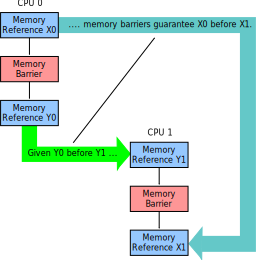
\includegraphics{memorder/memorybarrier}}
\caption{Memory Barriers Provide Conditional If-Then Ordering}
\label{fig:memorder:Memory Barriers Provide Conditional If-Then Ordering}
\end{figure}

\paragraph{Ordering has conditional if-then semantics.}
Figure~\ref{fig:memorder:Memory Barriers Provide Conditional If-Then Ordering}
illustrates this for memory barriers.
Assuming that both memory barriers are strong enough (and when in doubt, you
can always use \co{smp_mb()}), if CPU~1's access Y1 happens after CPU~0's
access Y0, then CPU~1's access X1 is guaranteed to happen after CPU~0's
access X1.

\QuickQuiz{}
	How can you tell which memory barriers are strong enough for
	a given use case?
\QuickQuizAnswer{
	Ah, that is a deep question whose answer requires most of the
	rest of this chapter.
} \QuickQuizEnd

Listing~\ref{lst:memorder:Memory Ordering: Store-Buffering Litmus Test}
is a case in point.
The \co{smp_mb()} on line~10 and~20 serve as the barriers,
the store to \co{x0} on line~9 as X0, the load from \co{x1} on line~11
as Y0, the store to \co{x1} on line~19 as Y1, and the load from
\co{x0} as X1.
Applying the if-then rule step by step, we know that the store to
\co{x1} on line~19 happens after the load from \co{x1} on line~11 if
\co{P0()}'s local variable \co{r2} is set to the value zero.
The if-then rule would then state that the load from \co{x0} on
line~21 happens after the store to \co{x0} on line~9.
In other words,
\co{P1()}'s local variable \co{r2} is guaranteed
to end up with the value two \emph{only if}
\co{P0()}'s local variable \co{r2} ends up with the value zero.
Again, memory ordering guarantees are conditional, not absolute.

Although
Figure~\ref{fig:memorder:Memory Barriers Provide Conditional If-Then Ordering}
specifically mentions memory barriers, the same rule applies to the
rest of the Linux kernel's ordering operations.

\paragraph{Ordering operations must be paired.}
If you carefully order the operations in one thread, but then fail to do
so in another thread, then there is no ordering.
Both threads must provide ordering for the if-then rule to apply.\footnote{
	In Section~\ref{sec:memorder:Propagation}, pairing will be
	generalized to cycles.}

\paragraph{Ordering operations almost never speed things up.}
If you find yourself tempted to add a memory barrier in an attempt
to force a prior store to be flushed to memory faster, resist!
Adding ordering usually slows things down.
Of course, there are situations where adding instructions speeds things
up, but careful benchmarking is required in such cases.
And even then, it is quite possible that although you sped things up
a little bit on \emph{your} system, you might well have slowed things
down significantly on your users' systems.
Or on your future system.

\paragraph{Ordering operations are not magic.}
When your program is failing due to some race condition, it is often
tempting to toss in a few memory-ordering operations in an attempt
to barrier your bugs out of existence.
A far better reaction is to use higher-level primitives in a carefully
designed manner.
With concurrent programming, it is almost always easier to design
your bugs out of existence than to hack them out of existence!

\paragraph{These are only rough rules of thumb.}
Although these rules of thumb cover the vast majority of situations
seen in actual practice, as with any set of rules of thumb, they
do have their limits.
The next section will demonstrate some of these limits by introducing
trick-and-trap litmus tests that are intended to insult your
intuition while increasing your understanding.
These litmus tests will also illuminate many of the concepts
represented by the Linux-kernel memory-ordering cheat sheet shown in
Table~\ref{tab:memorder:Linux-Kernel Memory-Ordering Cheat Sheet}.
Section~\ref{sec:memorder:Where is Memory Ordering Needed?} will
circle back to this cheat sheet in light of learnings from all the
intervening tricks and traps.

\section{Tricks and Traps}
\label{sec:memorder:Tricks and Traps}

Now that you know that hardware can reorder memory accesses and that you
can prevent it from doing so, the next step is to get you to admit
that your intuition has a problem.
This painful task is taken up by
Section~\ref{sec:memorder:Variables With Multiple Values},
which presents some code demonstrating that scalar variables can
take on multiple values simultaneously,
and by
Sections~\ref{sec:memorder:Memory-Reference Reordering} through
\ref{sec:memorder:Multicopy Atomicity},
which show a series of intuitively correct code fragments that fail miserably
on real hardware.
Once your intuition has made it through the grieving process, later
sections will summarize the basic rules that memory ordering follows.

But first, let's take a quick look at just how many values a single
variable might have at a single moment of time.

\subsection{Variables With Multiple Values}
\label{sec:memorder:Variables With Multiple Values}

It is natural to think of a variable as taking on a well-defined
sequence of values in a well-defined, global order.
Unfortunately, the next stop on the journey says ``goodbye'' to this comforting fiction.
Hopefully, you already started to say ``goodbye'' in response to row~2 of
Tables~\ref{tab:memorder:Memory Misordering: Store-Buffering Sequence of Events}
and~\ref{tab:memorder:Memory Ordering: Store-Buffering Sequence of Events},
and if so, the purpose of this section is to drive this point home.

To this end, consider the program fragment shown in
Listing~\ref{lst:memorder:Software Logic Analyzer}.
This code fragment is executed in parallel by several CPUs.
Line~1 sets a shared variable to the current CPU's ID, line~2
initializes several variables from a \co{gettb()} function that
delivers the value of a fine-grained hardware ``timebase'' counter that is
synchronized among all CPUs (not available from all CPU architectures,
unfortunately!), and the loop from lines~3-8 records the length of
time that the variable retains the value that this CPU assigned to it.
Of course, one of the CPUs will ``win'', and would thus never exit
the loop if not for the check on lines~6-7.

\QuickQuiz{}
	What assumption is the code fragment
	in Listing~\ref{lst:memorder:Software Logic Analyzer}
	making that might not be valid on real hardware?
\QuickQuizAnswer{
	The code assumes that as soon as a given CPU stops
	seeing its own value, it will immediately see the
	final agreed-upon value.
	On real hardware, some of the CPUs might well see several
	intermediate results before converging on the final value.
	The actual code used to produce the data in the figures
	discussed later in this section was therefore somewhat more
	complex.
} \QuickQuizEnd

\begin{listing}[tbp]
{ \scriptsize
\begin{verbbox}
  1 state.variable = mycpu;
  2 lasttb = oldtb = firsttb = gettb();
  3 while (state.variable == mycpu) {
  4   lasttb = oldtb;
  5   oldtb = gettb();
  6   if (lasttb - firsttb > 1000)
  7     break;
  8 }
\end{verbbox}
}
\centering
\theverbbox
\caption{Software Logic Analyzer}
\label{lst:memorder:Software Logic Analyzer}
\end{listing}

Upon exit from the loop, \co{firsttb} will hold a timestamp
taken shortly after the assignment and \co{lasttb} will hold
a timestamp taken before the last sampling of the shared variable
that still retained the assigned value, or a value equal to \co{firsttb}
if the shared variable had changed before entry into the loop.
This allows us to plot each CPU's view of the value of \co{state.variable}
over a 532-nanosecond time period, as shown in
Figure~\ref{fig:memorder:A Variable With Multiple Simultaneous Values}.
This data was collected in 2006 on 1.5\,GHz POWER5 system with 8 cores,
each containing a pair of hardware threads.
CPUs~1, 2, 3, and~4 recorded the values, while CPU~0 controlled the test.
The timebase counter period was about 5.32\,ns, sufficiently fine-grained
to allow observations of intermediate cache states.

\begin{figure}[htb]
\centering
\resizebox{3in}{!}{\includegraphics{memorder/MoreThanOneValue}}
\caption{A Variable With Multiple Simultaneous Values}
\label{fig:memorder:A Variable With Multiple Simultaneous Values}
\end{figure}

Each horizontal bar represents the observations of a given CPU over time,
with the black regions to the left indicating the time before the
corresponding CPU's first measurement.
During the first 5\,ns, only CPU~3 has an opinion about the value of the
variable.
During the next 10\,ns, CPUs~2 and~3 disagree on the value of the variable,
but thereafter agree that the value is~``2'', which is in fact
the final agreed-upon value.
However, CPU~1 believes that the value is~``1'' for almost 300\,ns, and
CPU~4 believes that the value is~``4'' for almost 500\,ns.

\QuickQuiz{}
	How could CPUs possibly have different views of the
	value of a single variable \emph{at the same time?}
\QuickQuizAnswer{
	As discussed in
	Section~\ref{sec:memorder:Why Hardware Misordering?},
	many CPUs have store buffers that record the values of
	recent stores, which do not become globally visible until
	the corresponding cache line makes its way to the CPU.
	Therefore, it is quite possible for each CPU to see a
	different value for a given variable at a single point
	in time---and for main memory to hold yet another value.
	One of the reasons that memory barriers were invented was
	to allow software to deal gracefully with situations like
	this one.
} \QuickQuizEnd

\QuickQuiz{}
	Why do CPUs~2 and~3 come to agreement so quickly, when it
	takes so long for CPUs~1 and~4 to come to the party?
\QuickQuizAnswer{
	CPUs~2 and~3 are a pair of hardware threads on the same
	core, sharing the same cache hierarchy, and therefore have
	very low communications latencies.
	This is a NUMA, or, more accurately, a NUCA effect.

	This leads to the question of why CPUs~2 and~3 ever disagree
	at all.
	One possible reason is that they each might have a small amount
	of private cache in addition to a larger shared cache.
	Another possible reason is instruction reordering, given the
	short 10-nanosecond duration of the disagreement and the
	total lack of memory-ordering operations in the code fragment.
} \QuickQuizEnd

And if you think that the situation with four CPUs was intriguing, consider
Figure~\ref{fig:memorder:A Variable With More Simultaneous Values},
which shows the same situation, but with 15~CPUs each assigning their
number to a single shared variable at time~$t=0$. Both diagrams in the
figure are drawn in the same way as
Figure~\ref{fig:memorder:A Variable With Multiple Simultaneous Values}.
The only difference is that the unit of horizontal axis is timebase ticks,
with each tick lasting about 5.3~nanoseconds.
The entire sequence therefore lasts a bit longer than the events recorded in
Figure~\ref{fig:memorder:A Variable With Multiple Simultaneous Values},
consistent with the increase in number of CPUs.
The upper diagram shows the overall picture, while the lower one shows
the zoom-up of first 50~timebase ticks.

Again, CPU~0 coordinates the test, so does not record any values.

\begin{figure*}
\centering
\resizebox{5in}{!}{\includegraphics{memorder/MoreThanOneValue-15CPU}}
\caption{A Variable With More Simultaneous Values}
\ContributedBy{Figure}{fig:memorder:A Variable With More Simultaneous Values}{Akira Yokosawa}
\end{figure*}

All CPUs eventually agree on the final value of~9, but not before
the values~15 and~12 take early leads.
Note that there are fourteen different opinions on the variable's value
at time~21 indicated by the vertical line in the lower diagram.
Note also that all CPUs see sequences whose orderings are consistent with
the directed graph shown in
Figure~\ref{fig:memorder:Possible Global Orders With More Simultaneous Values}.
Nevertheless, both figures underscore the importance of
proper use of memory-ordering operations, such as memory barriers,
for code that cares about memory ordering.

\begin{figure}[htb]
\centering
\resizebox{2.0in}{!}{\includegraphics{memorder/store15tred}}
\caption{Possible Global Orders With More Simultaneous Values}
\label{fig:memorder:Possible Global Orders With More Simultaneous Values}
\end{figure}

How many values can a single variable take on at a single point in
time?
As many as one per store buffer in the system!
We have therefore entered a regime where we must bid a fond farewell to
comfortable intuitions about values of variables and the passage of time.
This is the regime where memory-ordering operations are needed.

All that aside, it is important to remember the lessons from
Chapters~\ref{chp:Hardware and its Habits}
and~\ref{cha:Partitioning and Synchronization Design}.
Having all CPUs store concurrently to the same variable
is absolutely no way to design a parallel program, at least
not if performance and scalability are at all important to you.

Unfortunately, memory ordering has many other ways of insulting your
intuition, and not all of these ways conflict with performance and
scalability.
The next section will give an overview of reordering of unrelated
memory reference.

\subsection{Memory-Reference Reordering}
\label{sec:memorder:Memory-Reference Reordering}

Section~\ref{sec:memorder:Why Hardware Misordering?}
showed that even relatively strongly ordered systems like x86
can reorder prior stores with later loads, at least when the
store and load are to different variables.
This section builds on that result, looking at the other combinations of
loads and stores.

% @@@ Rationale for further reordering.

\begin{listing}[tbp]
{ \scriptsize
\begin{verbbox}[\LstLineNo]
C C-MP+o-wmb-o+o-o

{
}


P0(int* x0, int* x1) {

  WRITE_ONCE(*x0, 2);
  smp_wmb();
  WRITE_ONCE(*x1, 2);

}

P1(int* x0, int* x1) {

  int r2;
  int r3;

  r2 = READ_ONCE(*x1);
  r3 = READ_ONCE(*x0);

}

exists (1:r2=2 /\ 1:r3=0)
\end{verbbox}
}
\centering
\theverbbox
\caption{Message-Passing Litmus Test (No Ordering)}
\label{lst:memorder:Message-Passing Litmus Test (No Ordering)}
\end{listing}

\subsubsection{Load Followed By Load}
\label{sec:memorder:Load Followed By Load}

Listing~\ref{lst:memorder:Message-Passing Litmus Test (No Ordering)}
(\path{C-MP+o-wmb-o+o-o.litmus})
shows the classic \emph{message-passing} litmus test, where \co{x0} is
the message and \co{x1} is a flag indicating whether or not a message
is available.
In this test, the \co{smp_wmb()} forces \co{P0()} stores to be ordered,
but no ordering is specified for the loads.
Relatively strongly ordered architectures, such as x86, do enforce ordering.
However, weakly ordered architectures often do
not~\cite{JadeAlglave2011ppcmem}.
Therefore, the \co{exists} clause on line~25 of the listing \emph{can}
trigger.

\begin{listing}[tbp]
{ \scriptsize
\begin{verbbox}[\LstLineNo]
C C-MP+o-wmb-o+o-rmb-o

{
}

P0(int* x0, int* x1) {

  WRITE_ONCE(*x0, 2);
  smp_wmb();
  WRITE_ONCE(*x1, 2);

}

P1(int* x0, int* x1) {

  int r2;
  int r3;

  r2 = READ_ONCE(*x1);
  smp_rmb();
  r3 = READ_ONCE(*x0);

}

exists (1:r2=2 /\ 1:r3=0)
\end{verbbox}
}
\centering
\theverbbox
\caption{Enforcing Order of Message-Passing Litmus Test}
\label{lst:memorder:Enforcing Order of Message-Passing Litmus Test}
\end{listing}

Thus, portable code relying on ordering in this case must
add explicit ordering, for example, the \co{smp_rmb()} shown on
line~20 of
Listing~\ref{lst:memorder:Enforcing Order of Message-Passing Litmus Test}
(\path{C-MP+o-wmb-o+o-rmb-o.litmus}), which prevents
the \co{exists} clause from triggering.

\begin{listing}[tbp]
{ \scriptsize
\begin{verbbox}[\LstLineNo]
C C-LB+o-o+o-o
{
}

P0(int *x0, int *x1)
{
  int r2;

  r2 = READ_ONCE(*x1);
  WRITE_ONCE(*x0, 2);
}


P1(int *x0, int *x1)
{
  int r2;

  r2 = READ_ONCE(*x0);
  WRITE_ONCE(*x1, 2);
}

exists (1:r2=2 /\ 0:r2=2)
\end{verbbox}
}
\centering
\theverbbox
\caption{Load-Buffering Litmus Test (No Ordering)}
\label{lst:memorder:Load-Buffering Litmus Test (No Ordering)}
\end{listing}

\subsubsection{Load Followed By Store}
\label{sec:memorder:Load Followed By Store}

Listing~\ref{lst:memorder:Load-Buffering Litmus Test (No Ordering)}
(\path{C-LB+o-o+o-o.litmus})
shows the classic \emph{load-buffering} litmus test.
Although relatively strongly ordered systems such as x86
or the IBM Mainframe do not reorder prior loads with subsequent stores,
more weakly ordered architectures really do allow such
reordering~\cite{JadeAlglave2011ppcmem}.
Therefore, the \co{exists} clause on line~22 really can trigger.

\begin{listing}[tbp]
{ \scriptsize
\begin{verbbox}[\LstLineNo]
C C-LB+o-r+a-o
{
}

P0(int *x0, int *x1)
{
  int r2;

  r2 = READ_ONCE(*x1);
  smp_store_release(x0, 2);
}


P1(int *x0, int *x1)
{
  int r2;

  r2 = smp_load_acquire(x0);
  WRITE_ONCE(*x1, 2);
}

exists (1:r2=2 /\ 0:r2=2)
\end{verbbox}
}
\centering
\theverbbox
\caption{Enforcing Ordering of Load-Buffering Litmus Test}
\label{lst:memorder:Enforcing Ordering of Load-Buffering Litmus Test}
\end{listing}

Although it is rare for actual hardware to
exhibit this reordering~\cite{LucMaranget2017aarch64},
portable code must nevertheless enforce any required ordering, for example,
as shown in
Listing~\ref{lst:memorder:Enforcing Ordering of Load-Buffering Litmus Test}
(\path{C-LB+o-r+a-o.litmus}).
This guarantees that the \co{exists} clause on line~22 never triggers.

\begin{listing}[tbp]
{ \scriptsize
\begin{verbbox}[\LstLineNo]
C C-MP+o-o+o-rmb-o

{
}

P0(int* x0, int* x1) {

  WRITE_ONCE(*x0, 2);
  WRITE_ONCE(*x1, 2);

}

P1(int* x0, int* x1) {

  int r2;
  int r3;

  r2 = READ_ONCE(*x1);
  smp_rmb();
  r3 = READ_ONCE(*x0);

}

exists (1:r2=2 /\ 1:r3=0)
\end{verbbox}
}
\centering
\theverbbox
\caption{Message-Passing Litmus Test, No Writer Ordering (No Ordering)}
\label{lst:memorder:Message-Passing Litmus Test, No Writer Ordering (No Ordering)}
\end{listing}

\subsubsection{Store Followed By Store}
\label{sec:memorder:Store Followed By Store}

Listing~\ref{lst:memorder:Message-Passing Litmus Test, No Writer Ordering (No Ordering)}
(\path{C-MP+o-o+o-rmb-o.litmus})
once again shows the classic message-passing litmus test, but without
explicit ordering for \co{P0()}'s stores and with the \co{smp_rmb()}
providing ordering for \co{P1()}'s loads.
Again, the relatively strongly ordered architectures do enforce ordering,
but weakly ordered architectures do not necessarily do
so~\cite{JadeAlglave2011ppcmem}, which means that the
\co{exists} clause can trigger.
Therefore, portable code must explicitly order the stores, for
example, as shown in
Listing~\ref{lst:memorder:Enforcing Order of Message-Passing Litmus Test},
thus preventing the \co{exists} clause from triggering.

\subsection{Address Dependencies}
\label{sec:memorder:Address Dependencies}

An \emph{address dependency} occurs when the value returned by a load
instruction is used to compute the address used by a later memory-reference
instruction.

\begin{listing}[tbp]
{ \scriptsize
\begin{verbbox}[\LstLineNo]
C C-MP+o-wmb-o+o-addr-o

{
int y=1;
int *x1 = &y;
}

P0(int* x0, int** x1) {

  WRITE_ONCE(*x0, 2);
  smp_wmb();
  WRITE_ONCE(*x1, x0);

}

P1(int** x1) {

  int *r2;
  int r3;

  r2 = READ_ONCE(*x1);
  r3 = READ_ONCE(*r2);

}

exists (1:r2=x0 /\ 1:r3=1)
\end{verbbox}
}
\centering
\theverbbox
\caption{Message-Passing Address-Dependency Litmus Test (No Ordering)}
\label{lst:memorder:Message-Passing Address-Dependency Litmus Test (No Ordering)}
\end{listing}

Listing~\ref{lst:memorder:Message-Passing Address-Dependency Litmus Test (No Ordering)}
(\path{C-MP+o-wmb-o+o-addr-o.litmus}),
shows a linked variant of the message-passing pattern.
The head pointer is \co{x1}, which initially
references the \co{int} variable \co{y} (line~5), which is in turn
initialized to the value $1$ (line~4).
\co{P0()} updates head pointer \co{x1} to reference \co{x0} (line~12),
but only afer initializing it to $2$ (line~10) and forcing ordering
(line~11).
\co{P1()} picks up the head pointer \co{x1} (line~21), and then loads
the referenced value (line~22).
There is thus an address dependency from the load on line~21 to the
load on line~22.
In this case, the value returned by line~21 is exactly the address
used by line~22, but many variations are possible,
including field access using the C-language \co{->} operator,
addition, subtraction, and array indexing.

One might hope that line~21's load from the head pointer would be ordered
before line~22's dereference.
However, this is not the case on DEC Alpha, which can in effect use
a speculated value for the dependent load, as described in more detail in
Section~\ref{sec:memorder:Alpha}.
Therefore,
Listing~\ref{lst:memorder:Message-Passing Address-Dependency Litmus Test (No Ordering)}'s
\co{exists} clause \emph{can} trigger.

\begin{listing}[tbp]
{ \scriptsize
\begin{verbbox}[\LstLineNo]
C C-MP+o-wmb-o+ld-addr-o

{
int y=1;
int *x1 = &y;
}

P0(int* x0, int** x1) {

  WRITE_ONCE(*x0, 2);
  smp_wmb();
  WRITE_ONCE(*x1, x0);

}

P1(int** x1) {

  int *r2;
  int r3;

  r2 = lockless_dereference(*x1);
  r3 = READ_ONCE(*r2);

}

exists (1:r2=x0 /\ 1:r3=1)
\end{verbbox}
}
\centering
\theverbbox
\caption{Enforced Ordering of Message-Passing Address-Dependency Litmus Test}
\label{lst:memorder:Enforced Ordering of Message-Passing Address-Dependency Litmus Test}
\end{listing}

Listing~\ref{lst:memorder:Enforced Ordering of Message-Passing Address-Dependency Litmus Test}
(\path{C-MP+o-wmb-o+ld-addr-o.litmus})
shows how to make this work portably, even on DEC Alpha, by
replacing line~21's \co{READ_ONCE()} with \co{lockless_dereference()},
which acts like \co{READ_ONCE()} on all platforms other than DEC Alpha,
where it acts like a \co{READ_ONCE()} followed by an \co{smp_mb()},
thereby forcing the required ordering on all platforms, in turn
preventing the \co{exists} clause from triggering.

\begin{listing}[tbp]
{ \scriptsize
\begin{verbbox}[\LstLineNo]
C C-S+o-wmb-o+o-addr-o

{
int y=1;
int *x1 = &y;
}

P0(int* x0, int** x1) {

  WRITE_ONCE(*x0, 2);
  smp_wmb();
  WRITE_ONCE(*x1, x0);

}

P1(int** x1) {

  int *r2;

  r2 = READ_ONCE(*x1);
  WRITE_ONCE(*r2, 3);

}

exists (1:r2=x0 /\ x0=2)
\end{verbbox}
}
\centering
\theverbbox
\caption{S Address-Dependency Litmus Test}
\label{lst:memorder:S Address-Dependency Litmus Test}
\end{listing}

But what happens if the dependent operation is a store rather than
a load, for example, in the \emph{S}
litmus test~\cite{JadeAlglave2011ppcmem} shown in
Listing~\ref{lst:memorder:S Address-Dependency Litmus Test}
(\path{C-S+o-wmb-o+o-addr-o.litmus})?
Because no production-quality platform speculates stores,
it is not possible for the \co{WRITE_ONCE()} on line~10 to overwrite
the \co{WRITE_ONCE()} on line~21, meaning that the \co{exists}
clause on line~25 cannot trigger, even on DEC Alpha, even
without the \co{lockless_dereference()} that is required in the
dependent-load case.

\QuickQuiz{}
	But how do we know that \emph{all} platforms really avoid
	triggering the \co{exists} clauses in
	Listings~\ref{lst:memorder:Enforced Ordering of Message-Passing Address-Dependency Litmus Test}
	and~\ref{lst:memorder:S Address-Dependency Litmus Test}?
\QuickQuizAnswer{
	Answering this requires identifying three major groups of platforms:
	(1)~Total-store-order (TSO) platforms,
	(2)~Weakly ordered platorms, and
	(3)~DEC Alpha.

	The TSO platforms order all pairs of memory references except for
	prior stores against later loads.
	Because the address dependency on lines~21 and~22 of
	Listing~\ref{lst:memorder:Enforced Ordering of Message-Passing Address-Dependency Litmus Test}
	is instead a load followed by another load, TSO platforms preserve
	this address dependency.
	They also preserve the address dependency on lines~20 and~21 of
	Listing~\ref{lst:memorder:S Address-Dependency Litmus Test}
	because this is a load followed by a store.
	Because address dependencies must start with a load, TSO platforms
	implicitly but completely respect them.

	Weakly ordered platforms don't necessarily maintain ordering of
	unrelated accesses.
	However, the address dependencies in
	Listings~\ref{lst:memorder:Enforced Ordering of Message-Passing Address-Dependency Litmus Test}
	and~\ref{lst:memorder:S Address-Dependency Litmus Test}
	are not unrelated: There is an address dependency.
	The hardware tracks dependencies and maintains the needed
	ordering.

	There is one (famous) exception to this rule for weakly ordered
	platforms, and that exception is DEC Alpha for load-to-load
	address dependencies.
	And this is why DEC Alpha requires the explicit memory barrier
	supplied for it by the \co{lockless_dereference()} on line~21 of
	Listings~\ref{lst:memorder:Enforced Ordering of Message-Passing Address-Dependency Litmus Test}.
	However, DEC Alpha does track load-to-store address dependencies,
	which is why line~20 of
	Listings~\ref{lst:memorder:S Address-Dependency Litmus Test}
	does not have a \co{lockless_dereference()}.

	To sum up, current platforms either respect address dependencies
	implicitly, as is the case for TSO platforms (x86, mainframe,
	SPARC,~...), have hardware tracking for address dependencies
	(ARM, PowerPC, MIPS,~...), or have the required memory barriers
	supplied by \co{lockless_dereference()} (DEC Alpha).
} \QuickQuizEnd

However, it is important to note that address dependencies can
be fragile and easily broken by compiler optimizations, as discussed in
Section~\ref{sec:memorder:Address- and Data-Dependency Restrictions}.

\subsection{Data Dependencies}
\label{sec:memorder:Data Reordering}

A \emph{data dependency} occurs when the value returned by a load
instruction is used to compute the data stored by a later store
instruction.
Note well the ``data'' above: If the value returned by a load
was instead used to compute the address used by a later store
instruction, that would instead be an address dependency.

\begin{listing}[tbp]
{ \scriptsize
\begin{verbbox}[\LstLineNo]
C C-LB+o-r+o-data-o
{
}

P0(int *x0, int *x1)
{
  int r2;

  r2 = READ_ONCE(*x1);
  smp_store_release(x0, 2);
}


P1(int *x0, int *x1)
{
  int r2;

  r2 = READ_ONCE(*x0);
  WRITE_ONCE(*x1, r2);
}

exists (1:r2=2 /\ 0:r2=2)
\end{verbbox}
}
\centering
\theverbbox
\caption{Load-Buffering Data-Dependency Litmus Test}
\label{lst:memorder:Load-Buffering Data-Dependency Litmus Test}
\end{listing}

Listing~\ref{lst:memorder:Load-Buffering Data-Dependency Litmus Test}
(\path{C-LB+o-r+o-data-o.litmus})
is similar to
Listing~\ref{lst:memorder:Enforcing Ordering of Load-Buffering Litmus Test},
except that \co{P1()}'s ordering between lines~18 and~19 is
enforced not by an acquire load, but instead by a data dependency:
The value loaded by line~18 is what line~19 stores.
The ordering provided by this data dependency is sufficient to prevent
the \co{exists} clause from triggering.

\QuickQuiz{}
	Why doesn't line~18 of
	Listing~\ref{lst:memorder:Load-Buffering Data-Dependency Litmus Test}
	need a \co{lockless_dereference()}?
\QuickQuizAnswer{
	Data dependencies are always load-to-store dependencies, and
	so all platforms respect them, even DEC Alpha, and for the
	same reasons that they respect load-to-store address dependencies.
} \QuickQuizEnd

Just as with address dependencies, data dependencies are
fragile and can be easily broken by compiler optimizations, as discussed in
Section~\ref{sec:memorder:Address- and Data-Dependency Restrictions}.
In fact, data dependencies can be even more fragile than are address
dependencies.
The reason for this is that address dependencies normally involve
pointer values.
In contrast, as shown in
Listing~\ref{lst:memorder:Load-Buffering Data-Dependency Litmus Test},
it is tempting to carry data dependencies through integral values,
which the compiler has much more freedom to optimize into nonexistence.
For but one example, if the integer loaded was multiplied by the constant
zero, the compiler would know that the result was zero, and could therefore
substitute the constant zero for the value loaded, thus breaking
the dependency.

\QuickQuiz{}
	But wait!!!
	Line~18 of
	Listing~\ref{lst:memorder:Load-Buffering Data-Dependency Litmus Test}
	uses \co{READ_ONCE()}, which marks the load as volatile,
	which means that the compiler absolutely must emit the load
	instruction even if the value is later multiplied by zero.
	So do you really need to work so hard to keep the compiler from
	breaking your data dependencies?
\QuickQuizAnswer{
	Yes, the compiler absolutely must emit a load instruction for
	a volatile load.
	But if you multiply the value loaded by zero, the compiler is
	well within its rights to substitute a constant zero for the
	result of that multiplication, which will break the data
	dependency on many platforms.

	Worse yet, if the dependent store does not use \co{WRITE_ONCE()},
	the compiler could hoist it above the load, which would cause
	even TSO platforms to fail to provide ordering.
} \QuickQuizEnd

In short, you can rely on data dependencies, but only if you take care
to prevent your compiler from breaking them.

\subsection{Control Dependencies}
\label{sec:memorder:Control Dependencies}

A \emph{control dependency} occurs when the value returned by a load
instruction is tested to determine whether or not a later store instruction
is executed.
Note well the ``later store instruction'': Many platforms do not respect
load-to-load control dependencies.

\begin{listing}[tbp]
{ \scriptsize
\begin{verbbox}[\LstLineNo]
C C-LB+o-r+o-ctrl-o
{
}

P0(int *x0, int *x1)
{
  int r2;

  r2 = READ_ONCE(*x1);
  smp_store_release(x0, 2);
}


P1(int *x0, int *x1)
{
  int r2;

  r2 = READ_ONCE(*x0);
  if (r2 >= 0)
    WRITE_ONCE(*x1, 2);
}

exists (1:r2=2 /\ 0:r2=2)
\end{verbbox}
}
\centering
\theverbbox
\caption{Load-Buffering Control-Dependency Litmus Test}
\label{lst:memorder:Load-Buffering Control-Dependency Litmus Test}
\end{listing}

Listing~\ref{lst:memorder:Load-Buffering Control-Dependency Litmus Test}
(\path{C-LB+o-r+o-ctrl-o.litmus}),
shows another load-buffering example, this time using a control
dependency (line~19) to order the load on line~18 and the store on
line~20.
The ordering is sufficient to prevent the \co{exists} from triggering.

However, control dependencies are even more susceptible to being optimized
out of existence than are data dependencies, and
Section~\ref{sec:memorder:Control-Dependency Restrictions}
describes some of the rules that must be followed in order to prevent
your compiler from breaking your control dependencies.

\begin{listing}[tbp]
{ \scriptsize
\begin{verbbox}[\LstLineNo]
C C-MP+o-r+o-ctrl-o

{
}

P0(int* x0, int* x1) {

  WRITE_ONCE(*x0, 2);
  smp_store_release(x1, 2);

}

P1(int* x0, int* x1) {
  int r2;
  int r3 = 0;

  r2 = READ_ONCE(*x1);
  if (r2 >= 0)
    r3 = READ_ONCE(*x0);

}

exists (1:r2=2 /\ 1:r3=0)
\end{verbbox}
}
\centering
\theverbbox
\caption{Message-Passing Control-Dependency Litmus Test (No Ordering)}
\label{lst:memorder:Message-Passing Control-Dependency Litmus Test (No Ordering)}
\end{listing}

It is worth reiterating that control dependencies provide ordering only
from loads to stores.
Therefore, the load-to-load control dependency shown on lines~17-19 of
Listing~\ref{lst:memorder:Message-Passing Control-Dependency Litmus Test (No Ordering)}
(\path{C-MP+o-r+o-ctrl-o.litmus})
does \emph{not} provide ordering, and therefore does \emph{not}
prevent the \co{exists} clause from triggering.

In summary, control dependencies can be useful, but they are
high-maintenance items.
You should therefore use them only when performance considerations
permit no other solution.

\QuickQuiz{}
	Wouldn't control dependencies be more robust if they were
	mandated by language standards???
\QuickQuizAnswer{
	In the fullness of time, perhaps they will be so mandated.
} \QuickQuizEnd

\subsection{Cache Coherence}
\label{sec:memorder:Cache Coherence}

On cache-coherent platforms, all CPUs agree on the order of loads and
stores to a given variable.
Fortunately, when \co{READ_ONCE()} and \co{WRITE_ONCE()} are used,
almost all platforms are cache-coherent, as indicated by the ``SV''
column of the cheat sheet shown in
Table~\ref{tab:memorder:Linux-Kernel Memory-Ordering Cheat Sheet}.
Unfortunately, this property is so popular that it has been named
multiple times, with ``single-variable SC'',\footnote{
	Recall that SC stands for sequentially consistent.}
``single-copy atomic''~\cite{Stone:1995:SP:623262.623912},
and just plain ``coherence''~\cite{JadeAlglave2011ppcmem}
having seen use.
Rather than further compound the confusion by inventing yet another term
for this concept, this book uses ``cache coherence'' and ``coherence''
interchangeably.

\begin{listing}[tbp]
{ \scriptsize
\begin{verbbox}[\LstLineNo]
C C-CCIRIW+o+o+o-o+o-o

{
int x = 0;
}

P0(int *x)
{
  WRITE_ONCE(*x, 1);
}

P1(int *x)
{
  WRITE_ONCE(*x, 2);
}

P2(int *x)
{
  int r1;
  int r2;

  r1 = READ_ONCE(*x);
  r2 = READ_ONCE(*x);
}

P3(int *x)
{
  int r3;
  int r4;

  r3 = READ_ONCE(*x);
  r4 = READ_ONCE(*x);
}

exists(2:r1=1 /\ 2:r2=2 /\ 3:r3=2 /\ 3:r4=1)
\end{verbbox}
}
\centering
\theverbbox
\caption{Cache-Coherent IRIW Litmus Test}
\label{lst:memorder:Cache-Coherent IRIW Litmus Test}
\end{listing}

Listing~\ref{lst:memorder:Cache-Coherent IRIW Litmus Test}
(\path{C-CCIRIW+o+o+o-o+o-o.litmus})
shows a litmus test that tests for cache coherence,
where ``IRIW'' stands
for ``independent reads of independent writes''.
Because this litmus test uses only one variable,
\co{P2()} and \co{P3()} must agree
on the order of \co{P0()}'s and \co{P()}'s stores.
In other words, if \co{P2()} believes that \co{P0()}'s store
came first, then \co{P3()} had better not believe that
\co{P1()}'s store came first.
And in fact the \co{exists} clause on line~35 will trigger if this
situation arises.

It is tempting to speculate that different-sized overlapping loads
and stores to a single region of memory (as might be set up using
the C-language \co{union} keyword) would provide similar ordering
guarantees.
However, Flur et al.~discovered some surprisingly simple
litmus tests that demonstrate that these guarantees can be violated on
real hardware~\cite{Flur:2017:MCA:3093333.3009839}.
It is therefore necessary to restrict code to non-overlapping
same-sized aligned accesses to a given variable, at least if portability
is a consideration.\footnote{
	There is reason to believe that using atomic RMW operations
	(for example, \co{xchg()}) for all the stores will
	provide sequentially consistent ordering, but this has not
	yet been proven either way.}

Adding more variables and threads increases the scope for reordering
and other counterintuitive behavior, as discussed in the next section.

\subsection{Multicopy Atomicity}
\label{sec:memorder:Multicopy Atomicity}

\begin{figure}[tb]
\centering
\resizebox{3.0in}{!}{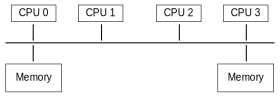
\includegraphics{memorder/SystemArchBus}}
\caption{Global System Bus And Multi-Copy Atomicity}
\label{fig:memorder:Global System Bus And Multi-Copy Atomicity}
\end{figure}

Threads running on a \emph{multicopy atomic}~\cite{Stone:1995:SP:623262.623912}
platform are guaranteed
to agree on the order of stores, even to different variables.
A useful mental model of such a system is the single-bus architecture
shown in
Figure~\ref{fig:memorder:Global System Bus And Multi-Copy Atomicity}.
If each store resulted in a message on the bus, and if the bus could
accommodate only one store at a time, then any pair of CPUs would
agree on the order of all stores that they observed.
Unfortunately, building a computer system as shown in the figure,
without store buffers or even caches, would result in glacial computation.
CPU vendors interested in providing multicopy atomicity have therefore
instead provided the slightly weaker
\emph{other-multicopy atomicity}~\cite[Section B2.3]{ARMv8A:2017},
which excludes the CPU doing a given store from the requirement that all
CPUs agree on the order of all stores.
This means that if only a subset of CPUs are doing stores, the
other CPUs will agree on the order of stores, hence the ``other''
in ``other-multicopy atomicity''.
Unlike multicopy-atomic platforms, within other-multicopy-atomic platforms,
the CPU doing the store is permitted to observe its
store early, which allows its later loads to obtain the newly stored
value directly from the store buffer.
This in turn avoids abysmal performance.

\QuickQuiz{}
	Can you give a specific example showing different behavior for
	multicopy atomic on the one hand and other-multicopy atomic
	on the other?
\QuickQuizAnswer{
\begin{listing}[tbp]
{ \scriptsize
\begin{verbbox}[\LstLineNo]
C C-MP-OMCA+o-o-o+o-rmb-o

{
}

P0(int *x, int *y)
{
  int r0;

  WRITE_ONCE(*x, 1);
  r0 = READ_ONCE(*x);
  WRITE_ONCE(*y, r0);
}

P1(int *x, int *y)
{
  int r1;
  int r2;

  r1 = READ_ONCE(*y);
  smp_rmb();
  r2 = READ_ONCE(*x);
}

exists (1:r1=1 /\ 1:r2=0)
\end{verbbox}
}
\centering
\theverbbox
\caption{Litmus Test Distinguishing Multicopy Atomic From Other Multicopy Atomic}
\label{lst:memorder:Litmus Test Distinguishing Multicopy Atomic From Other Multicopy Atomic}
\end{listing}

	Listing~\ref{lst:memorder:Litmus Test Distinguishing Multicopy Atomic From Other Multicopy Atomic}
	(\path{C-MP-OMCA+o-o-o+o-rmb-o.litmus})
	shows such a test.

	On a multicopy-atomic platform, \co{P0()}'s store to \co{x} on
	line~10 must become visible to both \co{P0()} and \co{P1()}
	simultaneously.
	Because this store becomes visible to \co{P0()} on line~11, before
	\co{P0()}'s store to \co{y} on line~12, \co{P0()}'s store to
	\co{x} must become visible before its store to \co{y} everywhere,
	including \co{P1()}.
	Therefore, if \co{P1()}'s load from \co{y} on line~20 returns the
	value 1, so must its load from \co{x} on line~22, given that
	the \co{smp_rmb()} on line~21 forces these two loads to execute
	in order.
	Therefore, the \co{exists} clause on line~25 cannot trigger on a
	multicopy-atomic platform.

	In contrast, on an other-multicopy-atomic platform, \co{P0()}
	could see its own store early, so that there would be no constraint
	on the order of visibility of the two stores from to \co{P1()},
	which in turn allows the \co{exists} clause to trigger.
} \QuickQuizEnd

Perhaps there will come a day when all platforms provide some flavor
of multi-copy atomicity, but
in the meantime, non-multicopy-atomic platforms do exist, and so software
does need to deal with them.

\begin{listing}[tbp]
{ \scriptsize
\begin{verbbox}[\LstLineNo]
C C-WRC-o+o-data-o+o-rmb-o

{
}

P0(int *x)
{
  WRITE_ONCE(*x, 1);
}

P1(int *x, int* y)
{
  int r1;

  r1 = READ_ONCE(*x);
  WRITE_ONCE(*y, r1);
}

P2(int *x, int* y)
{
  int r2;
  int r3;

  r2 = READ_ONCE(*y);
  smp_rmb();
  r3 = READ_ONCE(*x);
}

exists (1:r1=1 /\ 2:r2=1 /\ 2:r3=0)
\end{verbbox}
}
\centering
\theverbbox
\caption{WRC Litmus Test With Dependencies (No Ordering)}
\label{lst:memorder:WRC Litmus Test With Dependencies (No Ordering)}
\end{listing}

Listing~\ref{lst:memorder:WRC Litmus Test With Dependencies (No Ordering)}
(\path{C-WWC+o+o-data-o+o-addr-o.litmus})
demonstrates multicopy atomicity, that is, on a multicopy-atomic platform,
the \co{exists} clause on line~29 cannot trigger.
In contrast, on a non-multicopy-atomic
platform this \co{exists} clause can trigger, despite
\co{P1()}'s accesses being ordered by a data dependency and \co{P2()}'s
accesses being ordered by an \co{smp_rmb()}.
Recall that the definition of multicopy atomicity requires that all
threads agree on the order of stores, which can be thought of as
all stores reaching all threads at the same time.
Therefore, a non-multicopy-atomic platform can have a store reach
different threads at different times.
In particular, \co{P0()}'s store might reach \co{P1()} long before it
reaches \co{P2()}, which raises the possibility that \co{P1()}'s store
might reach \co{P2()} before \co{P0()}'s store does.

\begin{figure}[tb]
\centering
\resizebox{3.0in}{!}{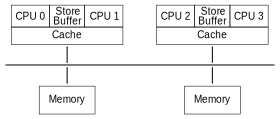
\includegraphics{memorder/NonMCAplatform}}
\caption{Shared Store Buffers And Multi-Copy Atomicity}
\label{fig:memorder:Shared Store Buffers And Multi-Copy Atomicity}
\end{figure}

This leads to the question of why a real system constrained by the
usual laws of physics would ever trigger the \co{exists} clause of
Listing~\ref{lst:memorder:WRC Litmus Test With Dependencies (No Ordering)}.
The cartoonish diagram of a such a real system is shown in
Figure~\ref{fig:memorder:Shared Store Buffers And Multi-Copy Atomicity}.
CPU~0 and CPU~1 share a store buffer, as do CPUs~2 and~3.
This means that CPU~1 can load a value out of the store buffer, thus
potentially immediately seeing a value stored by CPU~0.
In contrast, CPUs~2 and~3 will have to wait for the corresponding cache
line to carry this new value to them.

\QuickQuiz{}
	Then who would even \emph{think} of designing a system with shared
	store buffers???
\QuickQuizAnswer{
	This is in fact a very natural design for any system having
	multiple hardware threads per core.
	Natural from a hardware point of view, that is!
} \QuickQuizEnd

\begin{table*}
\small
\centering\OneColumnHSpace{-0.8in}
\begin{tabular}{r||l|l|l|l||l|l|l}
	& \tco{P0()} & \multicolumn{2}{c|}{\tco{P0()} \& \tco{P1()}} & \tco{P1()} & \multicolumn{3}{c}{\tco{P2()}} \\
	\cline{2-8}
	& Instruction & Store Buffer & Cache & Instruction &
			Instruction & Store Buffer & Cache \\
	\hline
	\hline
	1 & (Initial state) & & \tco{y==0} &
		(Initial state) &
			(Initial state) & & \tco{x==0} \\
	\hline
	2 & \tco{x = 1;} & \tco{x==1} & \tco{y==0} &
		 & & & \tco{x==0} \\
	\hline
	3 & (Read-Invalidate \tco{x}) & \tco{x==1} & \tco{y==0} & \tco{r1 = x} (1)
		 & & & \tco{x==0} \\
	\hline
	4 &  & \tco{x==1} \tco{y==1} & \tco{y==0} & \tco{y = r1}
		 & \tco{r2 = y} & & \tco{x==0} \\
	\hline
	5 &  & \tco{x==1} & \tco{y==1} & (Finish store)
		 & (Read \tco{y}) & & \tco{x==0} \\
	\hline
	6 & (Respond \tco{y}) & \tco{x==1} & \tco{y==1} &
		 & (\tco{r2==1}) & & \tco{x==0} \tco{y==1} \\
	\hline
	7 & & \tco{x==1} & \tco{y==1} &
		 & \tco{smp_rmb()} & & \tco{x==0} \tco{y==1} \\
	\hline
	8 & & \tco{x==1} & \tco{y==1} &
		 & \tco{r3 = x (0)} & & \tco{x==0} \tco{y==1} \\
	\hline
	9 & & \tco{x==1} & \tco{x==0} \tco{y==1} &
		 & (Respond \tco{x}) & & \tco{y==1} \\
	\hline
	10 & (Finish store) & & \tco{x==1} \tco{y==1} &
		 &  & & \tco{y==1} \\
\end{tabular}
\caption{Memory Ordering: WRC Sequence of Events}
\label{tab:memorder:Memory Ordering: WRC Sequence of Events}
\end{table*}

Table~\ref{tab:memorder:Memory Ordering: WRC Sequence of Events}
shows one sequence of events that can result in the \co{exists} clause in
Listing~\ref{lst:memorder:WRC Litmus Test With Dependencies (No Ordering)}
triggering.
This sequence of events will depend critically on \co{P0()} and
\co{P1()} sharing both cache and a store buffer in the manner shown in
Figure~\ref{fig:memorder:Shared Store Buffers And Multi-Copy Atomicity}.

\QuickQuiz{}
	But just how is it fair that P0 and P1 must share a store buffer
	and a cache, but P2 gets one each of its very own???
\QuickQuizAnswer{
	Presumably there is a P3, as is in fact shown in
	Figure~\ref{fig:memorder:Shared Store Buffers And Multi-Copy Atomicity},
	that shares P2's store buffer and cache.
	But not necessarily.
	Some platforms allow different cores to disable different numbers
	of threads, allowing the hardware to adjust to the needs of the
	workload at hand.
	For example, a single-threaded critical-path portion of the workload
	might be assigned to a core with only one thread enabled, thus
	allowing the single thread running that portion of the workload
	to use the entire capabilities of that core.
	Other more highly parallel but cache-miss-prone portions of the
	workload might be assigned to cores with all hardware threads
	enabled to provide improved throughput.
	This improved throughput could be due to the fact that while one
	hardware thread is stalled on a cache miss, the other hardware
	threads can make forward progress.

	In such cases, performance requirements override quaint human
	notions of fairness.
} \QuickQuizEnd

Row~1 shows the initial state, with the initial value of \co{y} in
P0's and P1's shared cache, and the initial value of \co{x} in
P2's cache.

Row~2 shows the immediate effect of \co{P0()} executing its store on line~8.
Because the cacheline containing \co{x} is not in \co{P0()}'s and \co{P1()}'s
shared cache, the new value (\co{1}) is stored in the shared store buffer.

Row~3 shows two transitions.
First, \co{P0()} issues a read-invalidate operation to fetch the cacheline
containing \co{x} so that it can flush the new value for \co{x} out of
the shared store buffer.
Second, \co{P1()} loads from \co{x} (line~15), an operation that completes
immediately because the new value of \co{x} is immediately available
from the shared store buffer.

Row~4 also shows two transitions.
First, it shows the immediate effect of \co{P1()} executing its store to
\co{y} (line~16), placing the new value into the shared store buffer.
Second, it shows the start of \co{P2()}'s load from \co{y} (line~24).

Row~5 continues the tradition of showing two transitions.
First, it shows \co{P1()} complete its store to \co{y}, flushing
from the shared store buffer to the cache.
Second, it shows \co{P2()} request the cacheline containing \co{y}.

Row~6 shows \co{P2()} receive the cacheline containing \co{y}, allowing
it to finish its load into \co{r2}, which takes on the value \co{1}.

Row~7 shows \co{P2()} execute its \co{smp_rmb()} (line~25), thus keeping
its two loads ordered.

Row~8 shows \co{P2()} execute its load from \co{x}, which immediately
returns with the value zero from \co{P2()}'s cache.

Row~9 shows \co{P2()} \emph{finally} responding to \co{P0()}'s request for
the cacheline containing \co{x}, which was made way back up on row~3.

Finally, row~10 shows \co{P0()} finish its store, flushing its value of
\co{x} from the shared store buffer to the shared cache.

Note well that the \co{exists} clause on line~29 has triggered.
The values of \co{r1} and \co{r2} are both the value one, and
the final value of \co{r3} the value zero.
This strange result occurred because \co{P0()}'s new value of \co{x} was
communicated to \co{P1()} long before it was communicated to \co{P2()}.

\QuickQuiz{}
	Referring to
	Table~\ref{tab:memorder:Memory Ordering: WRC Sequence of Events},
	why on earth would \co{P0()}'s store take so long to complete when
	\co{P1()}'s store complete so quickly?
	In other words, does the \co{exists} clause on line~32 of
	Listing~\ref{lst:memorder:WRC Litmus Test With Dependencies (No Ordering)}
	really trigger on real systems?
\QuickQuizAnswer{
	You need to face the fact that it really can trigger.
	Akira Yokosawa used the \co{litmus7} tool to run this litmus test
	on a Power8 system.
	Out of 1,000,000,000 runs, 4 triggered the \co{exists} clause.
	Thus, triggering the \co{exists} clause is not merely a one-in-a-million
	occurrence, but rather a one-in-a-hundred-million occurrence.
	But it nevertheless really does trigger on real systems.
} \QuickQuizEnd

This counter-intuitive result happens because although dependencies
do provide ordering, they provide it only within the confines of their
own thread.
This three-thread example requires stronger ordering, which
is the subject of
Sections~\ref{sec:memorder:Cumulativity}
through~\ref{sec:memorder:Release-Acquire Chains}.

\subsubsection{Cumulativity}
\label{sec:memorder:Cumulativity}

The three-thread example shown in
Listing~\ref{lst:memorder:WRC Litmus Test With Dependencies (No Ordering)}
requires \emph{cumulative} ordering, or \emph{cumulativity}.
A cumulative memory-ordering operation orders not just any given
access preceding it, but also earlier accesses by any thread to that
same variable.

\begin{listing}[tbp]
{ \scriptsize
\begin{verbbox}[\LstLineNo]
C C-WRC+o+o-r+a-o.litmus

{
}

P0(int *x)
{
  WRITE_ONCE(*x, 1);
}

P1(int *x, int* y)
{
  int r1;

  r1 = READ_ONCE(*x);
  smp_store_release(y, r1);
}

P2(int *x, int* y)
{
  int r2;
  int r3;

  r2 = smp_load_acquire(y);
  r3 = READ_ONCE(*x);
}

exists (1:r1=1 /\ 2:r2=1 /\ 2:r3=0)
\end{verbbox}
}
\centering
\theverbbox
\caption{WRC Litmus Test With Release}
\label{lst:memorder:WRC Litmus Test With Release}
\end{listing}

Dependencies do not provide cumulativity,
which is why the ``C'' column is blank for
both the \co{READ_ONCE()} and the \co{smp_read_barrier_depends()} rows
of Table~\ref{tab:memorder:Linux-Kernel Memory-Ordering Cheat Sheet}.
However, as indicated by the ``C'' in their ``C'' column,
release operations do provide cumulativity.
Therefore,
Listing~\ref{lst:memorder:WRC Litmus Test With Release}
(\path{C-WWC+o+o-r+o-addr-o.litmus})
substitutes a release operation for
Listing~\ref{lst:memorder:WRC Litmus Test With Dependencies (No Ordering)}'s
data dependency.
Because the release operation is cumulative, its ordering applies not only to
Listing~\ref{lst:memorder:WRC Litmus Test With Release}'s
load from \co{x} by \co{P1()} on line~15, but also to the store to \co{x}
by \co{P0()} on line~8---but only if that load returns the value stored,
which matches the \co{1:r1=1} in the \co{exists} clause on line~28.
This means that \co{P2()}'s load-acquire suffices to force the
load from \co{x} on line~25 to happen after the store on line~8, so
the value returned is one, which does not match \co{2:r3=0}, which
in turn prevents the \co{exists} clause from triggering.

\begin{figure*}[htbp]
\centering
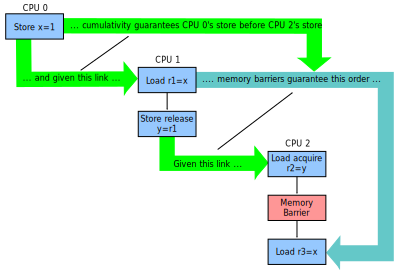
\includegraphics{memorder/memorybarriercum}
\caption{Cumulativity}
\label{fig:memorder:Cumulativity}
\end{figure*}

These ordering constraints are depicted graphically in
Figure~\ref{fig:memorder:Cumulativity}.
Note also that cumulativity is not limited to a single step back in time.
If there was another load from \co{x} or store to \co{x} from any thread
that came before the store on line~13, that prior load or store would also
be ordered before the store on line~32, though only if both \co{r1} and
\co{r2} both end up containing the address of \co{x}.

In short, use of cumulative ordering operations can suppress
non-multicopy-atomic behaviors in some situations.
Cumulativity nevertheless has limits, which are examined in the next section.

\subsubsection{Propagation}
\label{sec:memorder:Propagation}

\begin{listing}[tbp]
{ \scriptsize
\begin{verbbox}[\LstLineNo]
C C-W+RWC+o-r+a-o+o-mb-o

{
int x = 0;
int y = 0;
int z = 0;
}

P0(int *x, int *y)
{
  WRITE_ONCE(*x, 1);
  smp_store_release(y, 1);
}

P1(int *y, int *z)
{
  int r1;
  int r2;

  r1 = smp_load_acquire(y);
  r2 = READ_ONCE(*z);
}

P2(int *z, int *x)
{
  int r3;

  WRITE_ONCE(*z, 1);
  smp_mb();
  r3 = READ_ONCE(*x);
}

exists(1:r1=1 /\ 1:r2=0 /\ 2:r3=0)
\end{verbbox}
}
\centering
\theverbbox
\caption{W+RWC Litmus Test With Release (No Ordering)}
\label{lst:memorder:W+RWC Litmus Test With Release (No Ordering)}
\end{listing}

Listing~\ref{lst:memorder:W+RWC Litmus Test With Release (No Ordering)}
(\path{C-W+RWC+o-r+a-o+o-mb-o.litmus})
shows the limitations of cumulativity and of store-release,
even with a full memory barrier helping out.
The problem is that although the \co{smp_store_release()} on
line~12 has cumulativity, and although that cumulativity does
order \co{P2()}'s load on line~30, the \co{smp_store_release()}'s
ordering cannot propagate through the combination of \co{P1()}'s
load (line~21) and \co{P2()}'s store (line~28).
This means that the \co{exists} clause on line~33 really can trigger.

\QuickQuiz{}
	But it is not necessary to worry about propagation unless
	there are at least three threads in the litmus test, right?
\QuickQuizAnswer{
\begin{listing}[tbp]
{ \scriptsize
\begin{verbbox}[\LstLineNo]
C C-R+o-wmb-o+o-mb-o
{
}

P0(int *x0, int *x1)
{
  WRITE_ONCE(*x0, 1);
  smp_wmb();
  WRITE_ONCE(*x1, 1);
}


P1(int *x0, int *x1)
{
  int r2;

  WRITE_ONCE(*x1, 2);
  smp_mb();
  r2 = READ_ONCE(*x0);
}

exists (1:r2=0 /\ x1=2)
\end{verbbox}
}
\centering
\theverbbox
\caption{R Litmus Test With Write Memory Barrier (No Ordering)}
\label{lst:memorder:R Litmus Test With Write Memory Barrier (No Ordering)}
\end{listing}
	Wrong.

	Listing~\ref{lst:memorder:R Litmus Test With Write Memory Barrier (No Ordering)}
	(\path{C-R+o-wmb-o+o-mb-o.litmus})
	shows a two-thread litmus test that requires propagation due to
	the fact that it only has store-to-store and load-to-store
	links between its pair of threads.
	Even though \co{P0()} is fully ordered by the \co{smp_wmb()} and
	\co{P1()} is fully ordered by the \co{smp_mb()}, the
	counter-temporal nature of the links means that
	the \co{exists} clause on line~22 really can trigger.
	To prevent this triggering, the \co{smp_wmb()} on line~8
	must become an \co{smp_mb()}, bringing propagation into play
	twice, once for each non-temporal link.
} \QuickQuizEnd

\begin{figure}[htbp]
\centering
\resizebox{\columnwidth}{!}{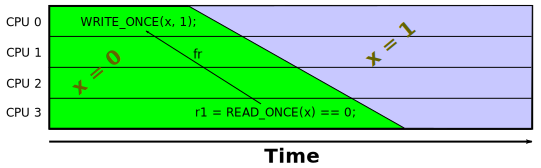
\includegraphics{memorder/fr}}
\caption{Load-to-Store is Counter-Temporal}
\label{fig:memorder:Load-to-Store is Counter-Temporal}
\end{figure}

This situation might seem completely counter-intuitive, but keep
in mind that the speed of light is finite and computers are of
non-zero size.
It therefore takes time for the effect of the \co{P2()}'s store to
\co{z} to propagate to \co{P1()}, which in turn means that it is possible
that \co{P1()}'s read from \co{z} happens much later in time, but
nevertheless still sees the old value of zero.
This situation is depicted in
Figure~\ref{fig:memorder:Load-to-Store is Counter-Temporal}:
Just because a load sees the old value does \emph{not} mean that
this load executed at an earlier time than did the store of the
new value.

Note that
Listing~\ref{lst:memorder:W+RWC Litmus Test With Release (No Ordering)}
also shows the limitations of memory-barrier pairing, given that
there are not two but three processes.
These more complex litmus tests can instead be said to have \emph{cycles},
where memory-barrier pairing is the special case of a two-thread cycle.
The cycle in
Listing~\ref{lst:memorder:W+RWC Litmus Test With Release (No Ordering)}
goes through \co{P0()} (lines~11 and~12), \co{P1()} (lines~20 and~21),
\co{P2()} (lines~28, 29, and~30), and back to \co{P0()} (line~11).
The \co{exists} clause delineates this cycle:
the \co{1:r1=1} indicates that the \co{smp_load_acquire()} on line~20
returned the value stored by the \co{smp_store_release()} on line~12,
the \co{1:r2=0} indicates that the \co{WRITE_ONCE()} on line~28 came
too late to affect the value returned by the \co{READ_ONCE()} on line~21,
and finally the \co{2:r3=0} indicates that the
\co{WRITE_ONCE()} on line~11 came too late to affect the value returned
by the \co{READ_ONCE()} on line~30.
In this case, the fact that the \co{exists} clause can trigger means that
the cycle is said to be \emph{allowed}.
In contrast, in cases where the \co{exists} clause cannot trigger,
the cycle is said to be \emph{prohibited}.

\begin{listing}[tbp]
{ \scriptsize
\begin{verbbox}[\LstLineNo]
C C-W+RWC+o-mb-o+a-o+o-mb-o

{
int x = 0;
int y = 0;
int z = 0;
}

P0(int *x, int *y)
{
  WRITE_ONCE(*x, 1);
  smp_mb();
  WRITE_ONCE(*y, 1);
}

P1(int *y, int *z)
{
  int r1;
  int r2;

  r1 = smp_load_acquire(y);
  r2 = READ_ONCE(*z);
}

P2(int *z, int *x)
{
  int r3;

  WRITE_ONCE(*z, 1);
  smp_mb();
  r3 = READ_ONCE(*x);
}

exists(1:r1=1 /\ 1:r2=0 /\ 2:r3=0)
\end{verbbox}
}
\centering
\theverbbox
\caption{W+WRC Litmus Test With More Barriers}
\label{lst:memorder:W+WRC Litmus Test With More Barriers}
\end{listing}

But what if we need to keep the \co{exists} clause on line~33 of
Listing~\ref{lst:memorder:W+RWC Litmus Test With Release (No Ordering)}?
One solution is to replace \co{P0()}'s \co{smp_store_release()}
with an \co{smp_mb()}, which
Table~\ref{tab:memorder:Linux-Kernel Memory-Ordering Cheat Sheet}
shows to have not only cumulativity, but also propagation.
The result is shown in
Listing~\ref{lst:memorder:W+WRC Litmus Test With More Barriers}
(\path{C-W+RWC+o-mb-o+a-o+o-mb-o.litmus}).

\QuickQuiz{}
	But given that \co{smp_mb()} has the propagation property,
	why doesn't the \co{smp_mb()} on line~29 of
	Listing~\ref{lst:memorder:W+RWC Litmus Test With Release (No Ordering)}
	prevent the \co{exists} clause from triggering?
\QuickQuizAnswer{
	As a rough rule of thumb, the \co{smp_mb()} barrier's
	propagation property is sufficient to maintain ordering
	through only one store-to-load link between
	processes.
	Unfortunately,
	Listing~\ref{lst:memorder:W+RWC Litmus Test With Release (No Ordering)}
	has not one but two store-to-load links, with the
	first being from the \co{READ_ONCE()} on line~21 to the
	\co{WRITE_ONCE()} on line~28 and the second being from
	the \co{READ_ONCE()} on line~30 to the \co{WRITE_ONCE()}
	on line~11.
	Therefore, preventing the \co{exists} clause from triggering
	should be expected to require not one but two
	instances of \co{smp_mb()}.

	As a special exception to this rule of thumb, a release-acquire
	chain can have one load-to-store link between processes
	and still prohibit the cycle.
} \QuickQuizEnd

\begin{figure}[tbp]
\centering
\resizebox{\columnwidth}{!}{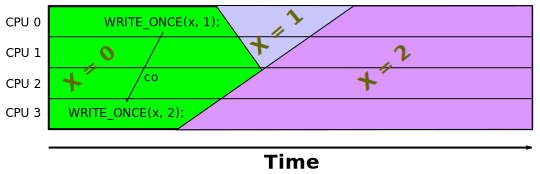
\includegraphics{memorder/co}}
\caption{Store-to-Store is Counter-Temporal}
\label{fig:memorder:Store-to-Store is Counter-Temporal}
\end{figure}

For completeness,
Figure~\ref{fig:memorder:Store-to-Store is Counter-Temporal}
shows that the ``winning'' store among a group of stores to the
same variable is not necessarily the store that started last.
This should not come as a surprise to anyone who carefully examined
Figure~\ref{fig:memorder:A Variable With More Simultaneous Values}.

But sometimes time is on our side, as shown in the next section.

\subsubsection{Happens-Before}
\label{sec:memorder:Happens-Before}

\begin{figure}[tbp]
\centering
\resizebox{\columnwidth}{!}{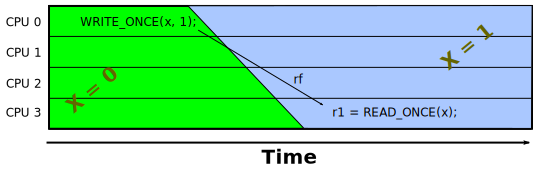
\includegraphics{memorder/rf}}
\caption{Store-to-Load is Temporal}
\label{fig:memorder:Store-to-Load is Temporal}
\end{figure}

As shown in
Figure~\ref{fig:memorder:Store-to-Load is Temporal},
on non-speculative platforms, if a load returns the value from a
particular store, then, courtesy of the finite speed of light and
the non-zero size of modern computing systems, the store absolutely
has to have executed at an earlier time than did the load.
This means that carefully constructed programs can rely on the
passage of time itself as an memory-ordering operation.

\begin{listing}[tbp]
{ \scriptsize
\begin{verbbox}[\LstLineNo]
C C-LB+a-o+o-data-o+o-data-o
{
}

P0(int *x0, int *x1)
{
  int r2;

  r2 = smp_load_acquire(x0);
  WRITE_ONCE(*x1, 2);
}


P1(int *x1, int *x2)
{
  int r2;

  r2 = READ_ONCE(*x1);
  WRITE_ONCE(*x2, r2);
}

P2(int *x2, int *x0)
{
  int r2;

  r2 = READ_ONCE(*x2);
  WRITE_ONCE(*x0, r2);
}

exists (0:r2=2 /\ 1:r2=2 /\ 2:r2=2)
\end{verbbox}
}
\centering
\theverbbox
\caption{LB Litmus Test With One Acquire}
\label{lst:memorder:LB Litmus Test With One Acquire}
\end{listing}

Of course, just the passage of time by itself is not enough, as
was seen in
Listing~\ref{lst:memorder:Load-Buffering Litmus Test (No Ordering)},
which has nothing but store-to-load links and still can
trigger its \co{exists} clause.
However, as long as each thread provides even the weakest possible
ordering, \co{exists} clause would not be able to trigger.
For example,
Listing~\ref{lst:memorder:LB Litmus Test With One Acquire}
(\path{C-LB+a-o+o-data-o+o-data-o.litmus})
shows \co{P0()} ordered with an \co{smp_load_acquire()} and
both \co{P1()} and \co{P2()} ordered with data dependencies.
These orderings, which are close to the top of
Table~\ref{tab:memorder:Linux-Kernel Memory-Ordering Cheat Sheet},
suffice to prevent the \co{exists} clause from triggering.

\QuickQuiz{}
	Can you construct a litmus test similar to that in
	Listing~\ref{lst:memorder:LB Litmus Test With One Acquire}
	that uses \emph{only} dependencies?
\QuickQuizAnswer{
	Listing~\ref{lst:memorder:LB Litmus Test With No Acquires}
	shows a somewhat nonsensical but very real example.
	Creating a more useful (but still real) litmus test is left
	as an exercise for the reader.
\begin{listing}[tbp]
{ \scriptsize
\begin{verbbox}[\LstLineNo]
C C-LB+o-data-o+o-data-o+o-data-o
{
int x0=0;
int x1=1;
int x2=2;
}

P0(int *x0, int *x1)
{
  int r2;

  r2 = READ_ONCE(*x0);
  WRITE_ONCE(*x1, r2);
}


P1(int *x1, int *x2)
{
  int r2;

  r2 = READ_ONCE(*x1);
  WRITE_ONCE(*x2, r2);
}

P2(int *x2, int *x0)
{
  int r2;

  r2 = READ_ONCE(*x2);
  WRITE_ONCE(*x0, r2);
}

exists (0:r2=2 /\ 1:r2=0 /\ 2:r2=1)
\end{verbbox}
}
\centering
\theverbbox
\caption{LB Litmus Test With No Acquires}
\label{lst:memorder:LB Litmus Test With No Acquires}
\end{listing}
} \QuickQuizEnd

An important, to say nothing of more useful, use of time for ordering
memory accesses is covered in the next section.

\subsubsection{Release-Acquire Chains}
\label{sec:memorder:Release-Acquire Chains}

\begin{listing}[tbp]
{ \scriptsize
\begin{verbbox}[\LstLineNo]
C C-LB+a-r+a-r+a-r+a-r
{
}

P0(int *x0, int *x1)
{
  int r2;

  r2 = smp_load_acquire(x0);
  smp_store_release(x1, 2);
}


P1(int *x1, int *x2)
{
  int r2;

  r2 = smp_load_acquire(x1);
  smp_store_release(x2, 2);
}

P2(int *x2, int *x3)
{
  int r2;

  r2 = smp_load_acquire(x2);
  smp_store_release(x3, 2);
}

P3(int *x3, int *x0)
{
  int r2;

  r2 = smp_load_acquire(x3);
  smp_store_release(x0, 2);
}

exists (0:r2=2 /\ 1:r2=2 /\ 2:r2=2 /\ 3:r2=2)
\end{verbbox}
}
\centering
\theverbbox
\caption{Long LB Release-Acquire Chain}
\label{lst:memorder:Long LB Release-Acquire Chain}
\end{listing}

A minimal release-acquire chain was shown in
Listing~\ref{lst:memorder:Enforcing Ordering of Load-Buffering Litmus Test}
(\path{C-LB+a-r+a-r+a-r+a-r.litmus}),
but these chains can be much longer, as shown in
Listing~\ref{lst:memorder:Long LB Release-Acquire Chain}.
The longer the release-acquire chain, the more benefit is gained
from the passage of time, so that no matter how many threads are
involved, the corresponding \co{exists} clause cannot trigger.
Give or take the increased computational demands of the larger number
of threads, of course!

\begin{listing}[tbp]
{ \scriptsize
\begin{verbbox}[\LstLineNo]
C C-ISA2+o-r+a-r+a-r+a-o
{
}

P0(int *x0, int *x1)
{
  WRITE_ONCE(*x0, 2);
  smp_store_release(x1, 2);
}


P1(int *x1, int *x2)
{
  int r2;

  r2 = smp_load_acquire(x1);
  smp_store_release(x2, 2);
}

P2(int *x2, int *x3)
{
  int r2;

  r2 = smp_load_acquire(x2);
  smp_store_release(x3, 2);
}

P3(int *x3, int *x0)
{
  int r1;
  int r2;

  r1 = smp_load_acquire(x3);
  r2 = READ_ONCE(*x0);
}

exists (1:r2=2 /\ 2:r2=2 /\ 3:r1=2 /\ 3:r2=0)
\end{verbbox}
}
\centering
\theverbbox
\caption{Long ISA2 Release-Acquire Chain}
\label{lst:memorder:Long ISA2 Release-Acquire Chain}
\end{listing}

Although release-acquire chains are inherently store-to-load creatures,
it turns out that they can tolerate one load-to-store step, despite
such steps being counter-temporal, as shown in
Figure~\ref{fig:memorder:Load-to-Store is Counter-Temporal}.
For example,
Listing~\ref{lst:memorder:Long ISA2 Release-Acquire Chain}
(\path{C-ISA2+o-r+a-r+a-r+a-o.litmus})
shows a three-step release-acquire chain, but where \co{P3()}'s
final access is a \co{READ_ONCE()} from \co{x0}, which is
accessed via \co{WRITE_ONCE()} by \co{P0()}, forming a non-temporal
load-to-store link between these two processes.
However, because \co{P0()}'s \co{smp_store_release()} (line~12)
is cumulative, if \co{P3()}'s \co{READ_ONCE()} returns zero,
this cumulativity will force the \co{READ_ONCE()} to be ordered
before \co{P0()}'s \co{smp_store_release()}.
In addition, the release-acquire chain (lines~12, 20, 21, 28, 29, and~37)
forces \co{P3()}'s \co{READ_ONCE()} to be ordered after \co{P0()}'s
\co{smp_store_release()}.
Because \co{P3()}'s \co{READ_ONCE()} cannot be both before and after
\co{P0()}'s \co{smp_store_release()}, either or both of two things must
be true:

\begin{enumerate}
\item	\co{P3()}'s \co{READ_ONCE()} came after \co{P0()}'s
	\co{WRITE_ONCE()}, so that the \co{READ_ONCE()} returned
	the value two, so that the \co{exists} clause's \co{3:r2=0}
	is false.
\item	The release-acquire chain did not form, that is, one or more
	of the \co{exists} clause's \co{1:r2=2}, \co{2:r2=2}, or \co{3:r1=2}
	is false.
\end{enumerate}

Either way, the \co{exists} clause cannot trigger, despite this litmus
test containing a notorious load-to-store link between
\co{P3()} and \co{P0()}.
But never forget that release-acquire chains can tolerate only one
load-to-store link, as was seen in
Listing~\ref{lst:memorder:W+RWC Litmus Test With Release (No Ordering)}.

\begin{listing}[tbp]
{ \scriptsize
\begin{verbbox}[\LstLineNo]
C C-Z6.2+o-r+a-r+a-r+a-o
{
}

P0(int *x0, int *x1)
{
  WRITE_ONCE(*x0, 2);
  smp_store_release(x1, 2);
}


P1(int *x1, int *x2)
{
  int r2;

  r2 = smp_load_acquire(x1);
  smp_store_release(x2, 2);
}

P2(int *x2, int *x3)
{
  int r2;

  r2 = smp_load_acquire(x2);
  smp_store_release(x3, 2);
}

P3(int *x3, int *x0)
{
  int r2;

  r2 = smp_load_acquire(x3);
  WRITE_ONCE(*x0, 3);
}

exists (1:r2=2 /\ 2:r2=2 /\ 3:r2=2 /\ x0=2)
\end{verbbox}
}
\centering
\theverbbox
\caption{Long Z6.2 Release-Acquire Chain}
\label{lst:memorder:Long Z6.2 Release-Acquire Chain}
\end{listing}

Release-acquire chains can also tolerate a single store-to-store step,
as shown in
Listing~\ref{lst:memorder:Long Z6.2 Release-Acquire Chain}
(\path{C-Z6.2+o-r+a-r+a-r+a-o.litmus}).
As with the previous example, \co{smp_store_release()}'s cumulativity
combined with the temporal nature of the release-acquire chain
prevents the \co{exists} clause on line~36 from triggering.
But beware: Adding a second store-to-store step would allow the correspondingly
updated \co{exists} clause to trigger.

% @@@ QQ on having a release-acquire chain with one load-to-store and
% @@@ one store-to-store link.

In short, properly constructed release-acquire chains form a peaceful
island of intuitive bliss surrounded by a strongly counter-intuitive
sea of more complex memory-ordering constraints.

% Exercises?
% Hardware details from Appendix?

\section{Compile-Time Consternation}
\label{sec:memorder:Compile-Time Consternation}

Most languages, including C, were developed on uniprocessor systems
by people with little or no parallel-programming experience.
As a results, unless explicitly told otherwise, these languages assume
that nothing else is reading or writing memory.
This in turn means that these languages' compilers' optimizers
are ready, willing, and oh so able to make dramatic changes to the
order, number, and sizes of memory references that your program
executes.
In fact, the reordering carried out by hardware can seem quite tame
by comparison.

This section will help you tame your compiler, thus avoiding a great
deal of compile-time consternation.
Section~\ref{sec:memorder:Memory-Reference Restrictions}
describes how to keep the compiler from destructively optimizing
your code's memory references,
Section~\ref{sec:memorder:Address- and Data-Dependency Restrictions}
describes how to protect address and data dependencies,
and finally,
Section~\ref{sec:memorder:Control-Dependency Restrictions}
describes how to protect those delicate control dependencies.

\subsection{Memory-Reference Restrictions}
\label{sec:memorder:Memory-Reference Restrictions}

Again, unless told otherwise, compilers assume that nothing else
is affecting the variables being accessed by the generated code.
This assumption is not simply some design error, but is instead enshrined in
various standards.\footnote{
	Or perhaps it is a standardized design error.}
This assumption means that compilers are within their rights
(as defined by the standards) to optimize the following code
so as to hoist the load from \co{a} out of the loop, at least
in cases where the compiler can prove that \co{do_something()}
does not modify \co{a}:

\vspace{5pt}
\begin{minipage}[t]{\columnwidth}
\scriptsize
\begin{verbatim}
  1 while (a)
  2   do_something();
\end{verbatim}
\end{minipage}
\vspace{5pt}

The optimized code might look something like this, essentially
fusing an arbitrarily large number of intended loads into a single
actual load:

\vspace{5pt}
\begin{minipage}[t]{\columnwidth}
\scriptsize
\begin{verbatim}
  1 if (a)
  2   for (;;)
  3     do_something();
\end{verbatim}
\end{minipage}
\vspace{5pt}

This optimization might come as a fatal surprise to code elsewhere
that expected to terminate this loop by storing a zero to \co{a}.
Prevent this by using \co{READ_ONCE()}, for example, as follows:

\vspace{5pt}
\begin{minipage}[t]{\columnwidth}
\scriptsize
\begin{verbatim}
  1 while (READ_ONCE(a))
  2   do_something();
\end{verbatim}
\end{minipage}
\vspace{5pt}

\co{READ_ONCE()} marks the load with a \co{volatile} cast.
Now \co{volatile} was originally designed for accessing
memory-mapped I/O (MMIO) registers, which are accessed using
the same load and store instructions that are used when
accessing normal memory.
However, MMIO registers need not act at all like normal memory.
Storing a value to an MMIO register does not necessarily mean
that a subsequent load from that register will return the value
stored.
Loading from an MMIO register might well have side effects,
for example, changing the device state or affecting the response
to subsequent loads and stores involving other MMIO registers.
Loads and stores of different sizes to the same MMIO address
might well have different effects.

This means that, even on a uniprocessor system, changing the
order, number, or size of MMIO accesses must be strictly
forbidden.
And this is exactly the purpose of the C-language \co{volatile} keyword,
to constrain the compiler to allow implementation of reliable device
drivers.

This is why \co{READ_ONCE()} prevents the destructive hoisting of
the load from \co{a} out of the loop:  Doing so changes the number
of \co{volatile} loads from \co{a}, so this optimization is disallowed.
However, note well that \co{volatile} does absolutely nothing to
constrain the hardware.
Therefore, if the code following the loop needs to see the result of
any memory references preceding the store of zero that terminated
the loop, you will instead need to use something like
\co{smp_store_release()} to store the zero and \co{smp_load_acquire()}
in the loop condition.
But if all you need is to reliably control the loop without any
other ordering, \co{READ_ONCE()} can do the job.

Compilers can also replicate loads.
For example, consider this all-too-real code fragment:

\vspace{5pt}
\begin{minipage}[t]{\columnwidth}
\scriptsize
\begin{verbatim}
  1 tmp = p;
  2 if (tmp != NULL && tmp <= q)
  3   do_something(tmp);
\end{verbatim}
\end{minipage}
\vspace{5pt}

Here the intent is that the \co{do_something()} function is never
passed a \co{NULL} pointer or a pointer that is greater than \co{q}.
However, the compiler is within its rights to transform this into the
following:

\vspace{5pt}
\begin{minipage}[t]{\columnwidth}
\scriptsize
\begin{verbatim}
  1 if (p != NULL && p <= q)
  2   do_something(p);
\end{verbatim}
\end{minipage}
\vspace{5pt}

In this transformed code, the value of \co{p} is loaded three
separate times.
This transformation might seem silly at first glance, but it is quite
tempting to compilers when the surrounding code has consumed all of the
machine registers.
It is possible that the current value of \co{p} passes the test on
line~1, but that some other thread stores \co{NULL} to \co{p} before
line~2 executes, and the resulting \co{NULL} pointer could be a fatal
surprise to \co{do_something()}.\footnote{
	Your editor made exactly this mistake in the DYNIX/ptx
	kernel's memory allocator in the early 1990s.
	Tracking down the bug consumed a holiday weekend not just
	for your editor, but also for several of his colleagues.
	In short, this is not a new problem.}

Compilers can also fuse stores.
The most infamous example is probably the progress-bar example
shown below:

\vspace{5pt}
\begin{minipage}[t]{\columnwidth}
\scriptsize
\begin{verbatim}
  1 while (!am_done()) {
  2   do_something(p);
  3   progress++;
  4 }
\end{verbatim}
\end{minipage}
\vspace{5pt}

If the compiler used a feedback-driven optimizer, it might well
notice that the store to the shared variable \co{progress} was
quite expensive, resulting in the following well-intentioned
optimization:

\vspace{5pt}
\begin{minipage}[t]{\columnwidth}
\scriptsize
\begin{verbatim}
  1 while (!am_done()) {
  2   do_something(p);
  3   tmp++;
  4 }
  5 progress = tmp;
\end{verbatim}
\end{minipage}
\vspace{5pt}

This might well slightly increase performance, but the poor user
watching the progress bar might be forgiven for harboring significant
ill will towards this particular optimization.
The progress bar will after all be stuck at zero for a long time,
then jump at the very end.
The following code will usually prevent this problem:

\vspace{5pt}
\begin{minipage}[t]{\columnwidth}
\scriptsize
\begin{verbatim}
  1 while (!am_done()) {
  2   do_something(p);
  3   WRITE_ONCE(progress, progress + 1);
  4 }
\end{verbatim}
\end{minipage}
\vspace{5pt}

Exceptions can occur if the compiler is able to analyze \co{do_something()}
and learn that it has no accesses to atomic or \co{volatile} variables.
In these cases the compiler could produce two loops, one invoking
\co{do_something()} and the other incrementing \co{progress}.
It may be necessary to replace the \co{WRITE_ONCE()} with something
like \co{smp_store_release()} in the unlikely event that this occurs.
It is important to note that although the compiler is forbidden from
changing the number, size, or order of \co{volatile} accesses, it is
perfectly within its rights to reorder normal accesses with unrelated
\co{volatile} accesses.

Oddly enough, the compiler is within its rights to use a variable
as temporary storage just before a store to that variable, thus
inventing stores to that variable.
Fortunately, most compilers avoid this sort of thing, at least outside
of stack variables.
Nevertheless, using \co{WRITE_ONCE()} (or declaring the variable
\co{volatile}) should prevent this sort of thing.
But take care: If you have a translation unit that uses that variable,
and never makes a volatile access to it, the compiler has no way of
knowing that it needs to be careful.

The previous examples involved compiler optimizations that
changed the number of accesses.
Now, it might seem that preventing the compiler from changing the
order of accesses is an act of futility, given that the underlying
hardware is free to reorder them.
However, modern machines have \emph{exact exceptions} and
\emph{exact interrupts}, meaning that any interrupt or exception will
appear to have happened at a specific place in the instruction
stream, so that the handler will see the effect of all prior
instructions, but won't see the effect of any subsequent instructions.
\co{READ_ONCE()} and \co{WRITE_ONCE()} can therefore be used to
control communication between interrupted code and interrupt handlers.

This leaves changes to the size of accesses, which is known as
\emph{load tearing} and \emph{store tearing} when the actual size
is smaller than desired.
For example, storing the constant \co{0x00010002} into a 32-bit
variable might seem quite safe.
However, there are CPUs that can store small immediate values
directly into memory, and on such CPUs, the compiler can be expected
to split this into two 16-bit stores in order to avoid the overhead
of explicitly forming the 32-bit constant.
This could come as a fatal surprise to another thread concurrently
loading from this variable, which might not expect to see the
result of a half-completed store.
Use of \co{READ_ONCE()} and \co{WRITE_ONCE()} prevent the compiler
from engaging in load tearing and store tearing, respectively.

In short, use of \co{READ_ONCE()}, \co{WRITE_ONCE()}, and
\co{volatile} are valuable tools in preventing the compiler from
optimizing your parallel algorithm out of existence.
Compilers are starting to provide other mechanisms for avoiding
load and store tearing, for example, \co{memory_order_relaxed}
atomic loads and stores, however, \co{volatile} is still needed
to avoid fusing and splitting of accesses.

\subsection{Address- and Data-Dependency Restrictions}
\label{sec:memorder:Address- and Data-Dependency Restrictions}

Compilers do not understand either address or data dependencies,
although there are efforts underway to teach them, or at the very
least, standardize the process of teaching
them~\cite{PaulEMcKennneyConsumeP0190R0,PaulEMcKenney2017markconsumeP0462R1}.
In the meantime, it is necessary to be very careful in order to avoid
giving your compiler the opportunity to break your dependencies.

\subsubsection{Give your dependency chain a good start}
The load that heads your dependency chain must use proper
ordering, for example, \co{lockless_dereference()},
\co{rcu_dereference()}, or
a \co{READ_ONCE()} followed by \co{smp_read_barrier_depends()}.
Failure to follow this rule can have serious side effects:

\begin{enumerate}
\item	On DEC Alpha, a dependent load might not be ordered with
	the load heading the dependency chain, as described in
	Section~\ref{sec:memorder:Alpha}.
\item	If the load heading the dependency chain is a
	C11 non-volatile \co{memory_order_relaxed} load,
	the compiler could omit the load, for example, by using a value
	that it loaded in the past.
\item	If the load heading the dependency chain is a plain load,
	the compiler can omit the load, again by using a value
	that it loaded in the past.
	Worse yet, it could load twice instead of once, so that
	different parts of your code use different values---and
	real compilers do this, especially when under register
	pressure.
\item	The value loaded by the head of the dependency chain must
	be a pointer.
	In theory, yes, you could load an integer, perhaps to use
	it as an array index.
	In practice, the compiler knows too much about integers,
	and thus has way too many opportunities to break your
	dependency chain.
\end{enumerate}

\subsubsection{Avoid arithmetic dependency breakage}
Although it is just fine to do some arithmetic operations on a pointer in
your dependency chain, you need to be careful to avoid giving the
compiler too much information.
After all, if the compiler learns enough to determine the exact value
of the pointer, it can and sometimes will use that exact value instead
of the pointer itself.
As soon as the compiler does that, the dependency is broken and all
ordering is lost.

\begin{listing}[tbp]
{ \scriptsize
\begin{verbbox}
 1 int reserve_int;
 2 int *gp;
 3 int *p;
 4
 5 p = rcu_dereference(gp);
 6 if (p == &reserve_int)
 7   handle_reserve(p);
 8 do_something_with(*p); /* buggy! */
\end{verbbox}
}
\centering
\theverbbox
\caption{Breakable Dependencies With Comparisons}
\label{lst:memorder:Breakable Dependencies With Comparisons}
\end{listing}

\begin{listing}[tbp]
{ \scriptsize
\begin{verbbox}
 1 int reserve_int;
 2 int *gp;
 3 int *p;
 4
 5 p = rcu_dereference(gp);
 6 if (p == &reserve_int) {
 7   handle_reserve(&reserve_int);
 8   do_something_with(reserve_int); /* buggy! */
 9 } else {
10   do_something_with(*p); /* OK! */
11 }
\end{verbbox}
}
\centering
\theverbbox
\caption{Broken Dependencies With Comparisons}
\label{lst:memorder:Broken Dependencies With Comparisons}
\end{listing}

\begin{enumerate}
\item	Although it is permissible to compute offsets from a
	pointer, these offsets must not result in total cancellation.
	For example, given a \co{char} pointer \co{cp},
	\co{cp-(uintptr_t)cp)} will cancel and can allow the compiler
	to break your dependency chain.
	On the other hand, canceling offset values with each other
	is perfectly safe and legal.
	For example, if \co{a} and \co{b} are equal, \co{cp+a-b}
	is an identity function, including preserving the dependency.
\item	Comparisons can break dependencies.
	Listing~\ref{lst:memorder:Breakable Dependencies With Comparisons}
	shows how this can happen.
	Here global pointer \co{gp} points to a dynamically allocated
	integer, but if memory is low, it might instead point to
	the \co{reserve_int} variable.
	This \co{reserve_int} case might need special handling, as
	shown on lines~6 and~7 of the figure.
	But the compiler could reasonably transform this code into
	the form shown in
	Listing~\ref{lst:memorder:Broken Dependencies With Comparisons},
	especially on systems where instructions with absolute
	addresses run faster than instructions using addresses
	supplied in registers.
	However, there is clearly no ordering between the pointer
	load on line~5 and the dereference on line~8.
	Please note that this is simply an example: There are a great
	many other ways to break dependency chains with comparisons.
\end{enumerate}

\QuickQuiz{}
	Why can't you simply dereference the pointer before comparing it
	to \co{&reserve_int} on line~6 of
	Listing~\ref{lst:memorder:Breakable Dependencies With Comparisons}?
\QuickQuizAnswer{
	For first, it might be necessary to invoke
	\co{handle_reserve()} before \co{do_something_with()}.

	But more relevant to memory ordering, the compiler is often within
	its rights to hoist the comparison ahead of the dereferences,
	which would allow the compiler to use \co{&reserve_int} instead
	of the varaiable \co{p} that the hardware has tagged with
	a dependency.
} \QuickQuizEnd

\QuickQuiz{}
	But it should be safe to compare two pointer variables,
	right?  After all, the compiler doesn't know the value
	of either, so how can it possibly learn anything from the
	comparison?
\QuickQuizAnswer{

\begin{listing}[tbp]
{ \scriptsize
\begin{verbbox}
 1 int *gp1;
 2 int *gp2;
 3 int *p;
 4 int *q;
 5
 6 p = rcu_dereference(gp1);
 7 q = READ_ONCE(gp2);
 8 if (p == q)
 9   handle_equality(p);
10 do_something_with(*p);
\end{verbbox}
}
\centering
\theverbbox
\caption{Breakable Dependencies With Non-Constant Comparisons}
\label{lst:memorder:Breakable Dependencies With Non-Constant Comparisons}
\end{listing}

\begin{listing}[tbp]
{ \scriptsize
\begin{verbbox}
 1 int *gp1;
 2 int *gp2;
 3 int *p;
 4 int *q;
 5
 6 p = rcu_dereference(gp1);
 7 q = READ_ONCE(gp2);
 8 if (p == q) {
 9   handle_equality(q);
10   do_something_with(*q);
11 } else {
12   do_something_with(*p);
13 }
\end{verbbox}
}
\centering
\theverbbox
\caption{Broken Dependencies With Non-Constant Comparisons}
\label{lst:memorder:Broken Dependencies With Non-Constant Comparisons}
\end{listing}

	Unfortunately, the compiler really can learn enough to
	break your dependency chain, for example, as shown in
	Listing~\ref{lst:memorder:Breakable Dependencies With Non-Constant Comparisons}.
	The compiler is within its rights to transform this code
	into that shown in
	Listing~\ref{lst:memorder:Broken Dependencies With Non-Constant Comparisons},
	and might well make this transformation due to register pressure
	if \co{handle_equality()} was inlined and needed a lot of registers.
	Line~10 of this transformed code uses \co{q}, which although
	equal to \co{p}, is not necessarily tagged by the hardware as
	carrying a dependency.
	Therefore, this transformed code does not necessarily guarantee
	that line~10 is ordered after line~6.\footnote{
		Kudos to Linus Torvalds for providing this example.}
} \QuickQuizEnd

% @@@ Quick quiz showing other ways to break dependencies by comparison

\subsubsection{Safe comparison of dependent pointers}
It turns out that there are several safe ways to compare dependent
pointers:

\begin{enumerate}
\item	Comparisons against the \co{NULL} pointer.
	In this case, all the compiler can learn is that the pointer
	is \co{NULL}, in which case you are not allowed to
	dereference it in any case.
\item	The dependent pointer is never dereferenced, whether before or
	after the comparison.
\item	The dependent pointer is compared to a pointer that references
	objects that were last modified a very long time ago, where
	the safest value of ``a very long time ago'' is at compile time.
\end{enumerate}

% @@@ convert to \co{uintptr_t} to set/clear bits and convert back.

% @@@ More here

In short, some care is required in order to ensure that dependency
chains in your source code are still dependency chains once the
compiler has gotten done with them.

\subsection{Control-Dependency Restrictions}
\label{sec:memorder:Control-Dependency Restrictions}

Control dependencies are especially tricky because current compilers
do not understand them and can easily break them.
The rules and examples in this section are intended to help you
prevent your compiler's ignorance from breaking your code.

A load-load control dependency requires a full read memory barrier,
not simply a data dependency barrier.
Consider the following bit of code:

\vspace{5pt}
\begin{minipage}[t]{\columnwidth}
\scriptsize
\begin{verbatim}
  1 q = READ_ONCE(x);
  2 if (q) {
  3   <data dependency barrier>
  4   q = READ_ONCE(y);
  5 }
\end{verbatim}
\end{minipage}
\vspace{5pt}

This will not have the desired effect because there is no actual data
dependency, but rather a control dependency that the CPU may short-circuit
by attempting to predict the outcome in advance, so that other CPUs see
the load from~\co{y} as having happened before the load from~\co{x}.
In such a case what's actually required is:

\vspace{5pt}
\begin{minipage}[t]{\columnwidth}
\scriptsize
\begin{verbatim}
  1 q = READ_ONCE(x);
  2 if (q) {
  3   <read barrier>
  4   q = READ_ONCE(y);
  5 }
\end{verbatim}
\end{minipage}
\vspace{5pt}

However, stores are not speculated.
This means that ordering \emph{is} provided for load-store control
dependencies, as in the following example:

\vspace{5pt}
\begin{minipage}[t]{\columnwidth}
\scriptsize
\begin{verbatim}
  1 q = READ_ONCE(x);
  2 if (q)
  3   WRITE_ONCE(y, 1);
\end{verbatim}
\end{minipage}
\vspace{5pt}

Control dependencies pair normally with other types of ordering operations.
That said, please note that neither \co{READ_ONCE()} nor \co{WRITE_ONCE()}
are optional!
Without the \co{READ_ONCE()}, the compiler might combine the load
from~\co{x} with other loads from~\co{x}.
Without the \co{WRITE_ONCE()}, the compiler might combine the store
to~\co{y} with other stores to~\co{y}.
Either can result in highly counterintuitive effects on ordering.

Worse yet, if the compiler is able to prove (say) that the value of
variable~\co{x} is always non-zero, it would be well within its rights
to optimize the original example by eliminating the ``\co{if}'' statement
as follows:

\vspace{5pt}
\begin{minipage}[t]{\columnwidth}
\scriptsize
\begin{verbatim}
  1 q = READ_ONCE(x);
  2 WRITE_ONCE(y, 1); /* BUG: CPU can reorder!!! */
\end{verbatim}
\end{minipage}
\vspace{5pt}

It is tempting to try to enforce ordering on identical stores on both
branches of the ``\co{if}'' statement as follows:

\vspace{5pt}
\begin{minipage}[t]{\columnwidth}
\scriptsize
\begin{verbatim}
 1 q = READ_ONCE(x);
 2 if (q) {
 3   barrier();
 4   WRITE_ONCE(y, 1);
 5   do_something();
 6 } else {
 7   barrier();
 8   WRITE_ONCE(y, 1);
 9   do_something_else();
10 }
\end{verbatim}
\end{minipage}
\vspace{5pt}

Unfortunately, current compilers will transform this as follows at high
optimization levels:

\vspace{5pt}
\begin{minipage}[t]{\columnwidth}
\scriptsize
\begin{verbatim}
 1 q = READ_ONCE(x);
 2 barrier();
 3 WRITE_ONCE(y, 1);  /* BUG: No ordering!!! */
 4 if (q) {
 5   do_something();
 6 } else {
 7   do_something_else();
 8 }
\end{verbatim}
\end{minipage}
\vspace{5pt}

Now there is no conditional between the load from~\co{x} and the store
to~\co{y}, which means that the CPU is within its rights to reorder them:
The conditional is absolutely required, and must be present in the
assembly code even after all compiler optimizations have been applied.
Therefore, if you need ordering in this example, you need explicit
memory-ordering operations, for example, a release store:

\vspace{5pt}
\begin{minipage}[t]{\columnwidth}
\scriptsize
\begin{verbatim}
 1 q = READ_ONCE(x);
 2 if (q) {
 3   smp_store_release(&y, 1);
 4   do_something();
 5 } else {
 6   smp_store_release(&y, 1);
 7   do_something_else();
 8 }
\end{verbatim}
\end{minipage}
\vspace{5pt}

The initial \co{READ_ONCE()} is still required to prevent the compiler from
proving the value of~\co{x}.

In addition, you need to be careful what you do with the local variable~%
\co{q},
otherwise the compiler might be able to guess the value and again remove
the needed conditional.
For example:

\vspace{5pt}
\begin{minipage}[t]{\columnwidth}
\scriptsize
\begin{verbatim}
 1 q = READ_ONCE(x);
 2 if (q % MAX) {
 3   WRITE_ONCE(y, 1);
 4   do_something();
 5 } else {
 6   WRITE_ONCE(y, 2);
 7   do_something_else();
 8 }
\end{verbatim}
\end{minipage}
\vspace{5pt}

If \co{MAX} is defined to be~1, then the compiler knows that \co{(q\%MAX)} is
equal to zero, in which case the compiler is within its rights to
transform the above code into the following:

\vspace{5pt}
\begin{minipage}[t]{\columnwidth}
\scriptsize
\begin{verbatim}
 1 q = READ_ONCE(x);
 2 WRITE_ONCE(y, 2);
 3 do_something_else();
\end{verbatim}
\end{minipage}
\vspace{5pt}

Given this transformation, the CPU is not required to respect the ordering
between the load from variable~\co{x} and the store to variable~\co{y}.
It is tempting to add a \co{barrier()} to constrain the compiler,
but this does not help.
The conditional is gone, and the \co{barrier()} won't bring it back.
Therefore, if you are relying on this ordering, you should make sure
that \co{MAX} is greater than one, perhaps as follows:

\vspace{5pt}
\begin{minipage}[t]{\columnwidth}
\scriptsize
\begin{verbatim}
 1 q = READ_ONCE(x);
 2 BUILD_BUG_ON(MAX <= 1);
 3 if (q % MAX) {
 4   WRITE_ONCE(y, 1);
 5   do_something();
 6 } else {
 7   WRITE_ONCE(y, 2);
 8   do_something_else();
 9 }
\end{verbatim}
\end{minipage}
\vspace{5pt}

Please note once again that the stores to~\co{y} differ.
If they were identical, as noted earlier, the compiler could pull this
store outside of the ``\co{if}'' statement.

You must also avoid excessive reliance on boolean short-circuit evaluation.
Consider this example:

\vspace{5pt}
\begin{minipage}[t]{\columnwidth}
\scriptsize
\begin{verbatim}
 1 q = READ_ONCE(x);
 2 if (q || 1 > 0)
 3   WRITE_ONCE(y, 1);
\end{verbatim}
\end{minipage}
\vspace{5pt}

Because the first condition cannot fault and the second condition is
always true, the compiler can transform this example as following,
defeating control dependency:

\vspace{5pt}
\begin{minipage}[t]{\columnwidth}
\scriptsize
\begin{verbatim}
 1 q = READ_ONCE(x);
 2 WRITE_ONCE(y, 1);
\end{verbatim}
\end{minipage}
\vspace{5pt}

This example underscores the need to ensure that the compiler cannot
out-guess your code.
More generally, although \co{READ_ONCE()} does force
the compiler to actually emit code for a given load, it does not force
the compiler to use the results.

In addition, control dependencies apply only to the then-clause and
else-clause of the if-statement in question.
In particular, it does
not necessarily apply to code following the if-statement:

\vspace{5pt}
\begin{minipage}[t]{\columnwidth}
\scriptsize
\begin{verbatim}
 1 q = READ_ONCE(x);
 2 if (q) {
 3   WRITE_ONCE(y, 1);
 4 } else {
 5   WRITE_ONCE(y, 2);
 6 }
 7 WRITE_ONCE(z, 1);  /* BUG: No ordering. */
\end{verbatim}
\end{minipage}
\vspace{5pt}

It is tempting to argue that there in fact is ordering because the
compiler cannot reorder volatile accesses and also cannot reorder
the writes to~\co{y} with the condition.
Unfortunately for this line
of reasoning, the compiler might compile the two writes to~\co{y} as
conditional-move instructions, as in this fanciful pseudo-assembly
language:

\vspace{5pt}
\begin{minipage}[t]{\columnwidth}
\scriptsize
\begin{verbatim}
 1 ld r1,x
 2 cmp r1,$0
 3 cmov,ne r4,$1
 4 cmov,eq r4,$2
 5 st r4,y
 6 st $1,z
\end{verbatim}
\end{minipage}
\vspace{5pt}

A weakly ordered CPU would have no dependency of any sort between the load
from~\co{x} and the store to~\co{z}.
The control dependencies would extend
only to the pair of cmov instructions and the store depending on them.
In short, control dependencies apply only to the stores in the ``\co{then}''
and ``\co{else}'' of the ``\co{if}'' in question (including functions
invoked by those two clauses), not to code following that ``\co{if}''.

Finally, control dependencies do \emph{not} provide cumulativity.\footnote{
	Refer to Section~\ref{sec:memorder:Cumulativity} for
	the meaning of cumulativity.}
This is demonstrated by two related examples, with the initial values
of~\co{x} and~\co{y} both being zero:

\vspace{5pt}
\begin{minipage}[t]{\columnwidth}
\tt
\scriptsize
\begin{tabular}{l|p{1.5in}}
	\nf{CPU 0} &	\nf{CPU 1} \\
	\hline
	\tco{r1 = READ_ONCE(x);} &
		\tco{r2 = READ_ONCE(y);} \\
	if (r1 > 0) &
		if (r2 > 0) \\
	~~~\tco{WRITE_ONCE(y, 1);} &
		~~~\tco{WRITE_ONCE(x, 1);} \\
	\multicolumn{2}{l}{~} \\
	\multicolumn{2}{l}{\tco{assert(!(r1 == 1 && r2 == 1));}} \\
\end{tabular}
\end{minipage}
\vspace{5pt}

The above two-CPU example will never trigger the \co{assert()}.
However, if control dependencies guaranteed transitivity (which they do
not), then adding the following CPU would guarantee a related assertion:

\vspace{5pt}
\begin{minipage}[t]{\columnwidth}
\tt
\scriptsize
\begin{tabular}{l}
	\nf{CPU 2} \\
	\hline
	\tco{WRITE_ONCE(x, 2);} \\
	\multicolumn{1}{l}{~} \\
	\multicolumn{1}{l}{\tco{assert(!(r1 == 2 && r2 == 1 && x == 2));}} \\
\end{tabular}
\end{minipage}
\vspace{5pt}

But because control dependencies do \emph{not} provide transitivity, the above
assertion can fail after the combined three-CPU example completes.
If you need the three-CPU example to provide ordering, you will need
\co{smp_mb()} between the loads and stores in the CPU~0 and CPU~1 code
fragments, that is, just before or just after the ``\co{if}'' statements.
Furthermore, the original two-CPU example is very fragile and should be avoided.

The two-CPU example is known as LB (load buffering) and the three-CPU
example as WWC~\cite{Maranget2012TutorialARMPower}.

The following list of rules summarizes the lessons of this section:

\begin{enumerate}
\item	Compilers do not understand control dependencies, so it is
	your job to make sure that the compiler cannot break your code.

\item	Control dependencies can order prior loads against later stores.
	However, they do \emph{not} guarantee any other sort of ordering:
	Not prior loads against later loads, nor prior stores against
	later anything.
	If you need these other forms of ordering, use \co{smp_rmb()},
	\co{smp_wmb()}, or, in the case of prior stores and later loads,
	\co{smp_mb()}.

\item	If both legs of the ``\co{if}'' statement begin with identical stores
	to the same variable, then those stores must be ordered,
	either by preceding both of them with \co{smp_mb()} or by using
	\co{smp_store_release()} to carry out the stores.
	Please note that it is \emph{not} sufficient to use \co{barrier()}
	at beginning of each leg of the ``\co{if}'' statement because, as shown
	by the example above, optimizing compilers can destroy the control
	dependency while respecting the letter of the \co{barrier()} law.

\item	Control dependencies require at least one run-time conditional
	between the prior load and the subsequent store, and this
	conditional must involve the prior load.
	If the compiler is able to optimize the conditional away, it
	will have also optimized away the ordering.
	Careful use of \co{READ_ONCE()} and \co{WRITE_ONCE()} can help
	to preserve the needed conditional.

\item	Control dependencies require that the compiler avoid reordering
	the dependency into nonexistence.
	Careful use of \co{READ_ONCE()}, \co{atomic_read()}, or
	\co{atomic64_read()} can help to preserve your control
	dependency.

\item	Control dependencies apply only to the ``\co{then}'' and
	``\co{else}'' of the ``\co{if}'' containing the control
	dependency, including any functions that these two clauses call.
	Control dependencies do \emph{not} apply to code following the
	``\co{if}'' containing the control dependency.

\item	Control dependencies pair normally with other types of
	memory-ordering operations.

\item	Control dependencies do \emph{not} provide transitivity.
	If you need transitivity, use \co{smp_mb()}.
\end{enumerate}

In short, many popular languages were designed primarily with
single-threaded use in mind.
Successfully using these languages to construct multi-threaded software
requires that you pay special attention to your memory references and
dependencies.

\section{Hardware Specifics}
\label{sec:memorder:Hardware Specifics}
\OriginallyPublished{Appendix}{sec:memorder:Hardware Specifics}{Memory-Barrier Instructions For Specific CPUs}{Linux Journal}{PaulMcKenney2005i,PaulMcKenney2005j}

\begin{table*}
\small
\centering
\renewcommand*{\arraystretch}{1.2}\OneColumnHSpace{-.6in}
\begin{tabular}{l|p{2in}|c|c|c|c|c|c|c|c|c|c|c}
	\multicolumn{2}{l|}{~}
	& \begin{picture}(6,60)(0,0)
		\rotatebox{90}{Alpha}
	  \end{picture}
	& \begin{picture}(6,60)(0,0)
		\rotatebox{90}{ARMv8}
	  \end{picture}
	& \begin{picture}(6,60)(0,0)
		\rotatebox{90}{ARMv7-A/R}
	  \end{picture}
	& \begin{picture}(6,60)(0,0)
		\rotatebox{90}{Itanium}
	  \end{picture}
	& \begin{picture}(6,60)(0,0)
		\rotatebox{90}{MIPS}
	  \end{picture}
	& \begin{picture}(6,60)(0,0)
		\rotatebox{90}{(PA-RISC)}
	  \end{picture}
	& \begin{picture}(6,60)(0,0)
		\rotatebox{90}{PA-RISC CPUs}
	  \end{picture}
	& \begin{picture}(6,60)(0,0)
		\rotatebox{90}{POWER}
	  \end{picture}
	& \begin{picture}(6,60)(0,0)
		\rotatebox{90}{SPARC TSO}
	  \end{picture}
	& \begin{picture}(6,60)(0,0)
		\rotatebox{90}{x86}
	  \end{picture}
	& \begin{picture}(6,60)(0,0)
		\rotatebox{90}{z~Systems}
	  \end{picture}
	\\
	\hline
%		 Alpha ARMv8 ARMv7 Itanium MIPS PA-RISC -CPUs PPC SPARC x86 z Systems
	\hline
        Memory Ordering
	& Loads Reordered After Loads or Stores?
		 & Y   & Y   & Y   & Y     & Y  & Y     & ~   & Y & ~   & ~ & ~ \\
	\cline{2-13}
	& Stores Reordered After Stores?
		 & Y   & Y   & Y   & Y     & Y  & Y     & ~   & Y & ~   & ~ & ~ \\
	\cline{2-13}
	& Stores Reordered After Loads?
		 & Y   & Y   & Y   & Y     & Y  & Y     & ~   & Y & Y   & Y & Y \\
	\cline{2-13}
	& Atomic Instructions Reordered With Loads or Stores?
		 & Y   & Y   & Y   & ~     & Y  & ~     & ~   & Y & ~   & ~ & ~ \\
	\cline{2-13}
	& Dependent Loads Reordered?
		 & Y   & ~   & ~   & ~     & ~  & ~     & ~   & ~ & ~   & ~ & ~ \\
	\cline{2-13}
	& Dependent Stores Reordered?
		 & ~   & ~   & ~   & ~     & ~  & ~     & ~   & ~ & ~   & ~ & ~ \\
	\cline{2-13}
	& Non-Sequentially Consistent?
		 & Y   & Y   & Y   & Y     & Y  & Y     & ~   & Y & Y   & Y & Y \\
	\cline{2-13}
	& Non-Multicopy Atomic?
		 & Y   & Y   & Y   & Y     & Y  & Y     & ~   & Y & Y   & Y & ~ \\
	\cline{2-13}
	& Non-Other-Multicopy Atomic?
		 & Y   & ~   & Y   & Y     & Y  & Y     & ~   & Y & Y   & Y & ~ \\
	\cline{2-13}
	& Non-Cache Coherent?
		 & ~   & ~   & ~   & Y     & ~  & ~     & ~   & ~ & ~   & ~ & ~ \\
	\hline
        \hline
        Instructions
	& Load-Acquire/Store-Release?
		 & F   & i   & F   & I     & ?  & ?     & ~   & b & ~   & ~ & ~ \\
        \cline{2-13}
	& Atomic RMW Instruction Type?
		 & L   & L   & L   & C     & L  & ?     & ?   & L & ?   & C & C \\
        \cline{2-13}
	& Incoherent Instruction Cache/Pipeline?
		 & Y   & Y   & Y   & Y     & Y  & ~     & ~   & Y & Y   & Y & Y \\
\end{tabular}
\renewcommand*{\arraystretch}{1}
\begin{tabular}{llcl}
	~ & ~ & ~ & ~\\
	{ \bf Key: } & ~ & ~ & ~ \\
	~ & \multicolumn{3}{l}{Load-Acquire/Store-Release?} \\
	~ & ~ & b: & Lightweight memory barrier \\
	~ & ~ & F: & Full memory barrier \\
	~ & ~ & i: & Instruction with lightweight ordering \\
	~ & ~ & I: & Instruction with heavyweight ordering \\
	~ &\multicolumn{3}{l}{Atomic RMW Instruction Type?} \\
	~ & ~ & C: & Compare-and-exchange instruction \\
	~ & ~ & L: & Load-linked/store-conditional instruction \\
\end{tabular}
\caption{Summary of Memory Ordering}
\label{tab:memorder:Summary of Memory Ordering}
\end{table*}

Each CPU has its own peculiar approach to memory ordering, which
can make portability a challenge, as indicated by
Table~\ref{tab:memorder:Summary of Memory Ordering}.
In fact, some software environments simply prohibit
direct use of memory-ordering operations, restricting the programmer
to mutual-exclusion primitives that incorporate them to the extent that
they are required.  Please note that this section is not intended to be
a reference manual
covering all (or even most) aspects of each CPU family, but rather
a high-level overview giving a rough comparison.
For full details, see the reference manual for the CPU of interest.

Getting back to
Table~\ref{tab:memorder:Summary of Memory Ordering},
the first group of rows look at memory-ordering
properties and the second group looks at instruction properties.

The first three rows indicate whether a given CPU allows the four
possible combinations of loads and stores to be reordered, as discussed
in
Sections~\ref{sec:memorder:Ordering: Why and How?} and
\ref{sec:memorder:Load Followed By Load}--\ref{sec:memorder:Store Followed By Store}.
The next row (``Atomic Instructions Reordered With Loads or Stores?'')
indicates whether a given CPU allows loads and stores
to be reordered with atomic instructions.

The fifth and sixth rows cover reordering and dependencies,
which was covered in
Sections~\ref{sec:memorder:Address Dependencies}--\ref{sec:memorder:Control Dependencies}
and which is explained in more detail in
Section~\ref{sec:memorder:Alpha}.
The short version is that Alpha requires memory barriers for readers
as well as updaters of linked data structures.

The next row, ``Non-Sequentially Consistent'', indicates whether
the CPU's normal load and store instructions are constrained by
sequential consistency.
Almost all are not constrained in this way for performance reasons.

The next two rows cover multicopy atomicity, which was defined in
Section~\ref{sec:memorder:Multicopy Atomicity}.
The first is full-up (and rare) multicopy atomicity, and the second is the
weaker other-multicopy atomicity.

The next row, ``Non-Cache Coherent'', covers accesses from multiple
threads to a single variable, which was discussed in
Section~\ref{sec:memorder:Cache Coherence}.

The final three rows cover instruction-level choices and issues.
The first row indicates how each CPU implements load-acquire
and store-release, the second row classifies CPUs by atomic-instruction
type, and the third and final row
indicates whether a given CPU has an incoherent
instruction cache and pipeline.
Such CPUs require special instructions be executed for self-modifying
code.

Parenthesized CPU names indicate modes that are architecturally allowed,
but rarely used in practice.

The common ``just say no'' approach to memory-ordering operations
can be eminently reasonable where it applies,
but there are environments, such as the Linux kernel, where direct
use of memory-ordering operations is required.
Therefore,
Linux provides a carefully chosen least-common-denominator
set of memory-ordering primitives, which are as follows:
\begin{description}
\item	[\tco{smp_mb()}] (full memory barrier) that orders both loads and
	stores.
	This means that loads and stores preceding the memory barrier
	will be committed to memory before any loads and stores
	following the memory barrier.
\item	[\tco{smp_rmb()}] (read memory barrier) that orders only loads.
\item	[\tco{smp_wmb()}] (write memory barrier) that orders only stores.
\item	[\tco{smp_read_barrier_depends()}] that forces subsequent operations
	that depend on prior operations to be ordered.
	This primitive is a no-op on all platforms except Alpha, but
	is normally not used directly, but rather as part of
	something like \co{lockless_dereference()} or
	\co{rcu_dereference()}.
\item	[\tco{smp_mb__before_atomic()}] that forces ordering of accesses
	preceding the \co{smp_mb__before_atomic()} against accesses following
	a later RMW atomic operation.
	This is a noop on systems that fully order atomic RMW operatings.
\item	[\tco{smp_mb__after_atomic()}] that forces ordering of accesses
	preceding an earlier RMW atomic operation against accesses
	following the \co{smp_mb__after_atomic()}.
	This is also a noop on systems that fully order atomic RMW operatings.
\item	[\tco{mmiowb()}] that forces ordering on MMIO writes that are guarded
	by global spinlocks, and is more thoroughly described
	in a 2016 LWN article on MMIO~\cite{PaulEMcKenney2016LinuxKernelMMIO}.
\end{description}
The \co{smp_mb()}, \co{smp_rmb()}, and \co{smp_wmb()}
primitives also force
the compiler to eschew any optimizations that would have the effect
of reordering memory optimizations across the barriers.
The \co{smp_read_barrier_depends()} primitive has a similar effect, but
only on Alpha CPUs.

These primitives generate code only in SMP kernels, however, each
also has a UP version ({\tt mb()}, {\tt rmb()}, {\tt wmb()},
and \co{read_barrier_depends()},
respectively) that generate a memory barrier even in UP kernels. The \co{smp_}
versions should be used in most cases. However, these latter primitives
are useful when writing drivers, because MMIO accesses must remain
ordered even in UP kernels. In absence of memory-ordering operations,
both CPUs and compilers would happily rearrange these accesses, which at
best would make the device act strangely, and could crash your kernel or,
in some cases, even damage your hardware.

So most kernel programmers need not worry about the memory-ordering
peculiarities of each and every CPU, as long as they stick to these
interfaces.
If you are working deep in a given CPU's architecture-specific code,
of course, all bets are off.

Furthermore,
all of Linux's locking primitives (spinlocks, reader-writer locks,
semaphores, RCU, \ldots) include any needed ordering primitives.
So if you are working with code that uses these primitives, you don't
even need to worry about Linux's memory-ordering primitives.

That said, deep knowledge of each CPU's memory-consistency model
can be very helpful when debugging, to say nothing of when writing
architecture-specific code or synchronization primitives.

Besides, they say that a little knowledge is a very dangerous thing.
Just imagine the damage you could do with a lot of knowledge!
For those who wish to understand more about individual CPUs'
memory consistency models, the next sections describes those of the
most popular and prominent CPUs.
Although nothing can replace actually reading a given CPU's documentation,
these sections give a good overview.

\subsection{Alpha}
\label{sec:memorder:Alpha}

It may seem strange to say much of anything about a CPU whose end of life
has long since past, but Alpha is interesting because, with one of
the weakest memory ordering models, it reorders memory operations quite
aggressively.
It therefore has defined many of the Linux-kernel memory-ordering primitives,
which must work on all CPUs, including Alpha.
Understanding Alpha is therefore surprisingly important to the Linux kernel
hacker.

The difference between Alpha and the other CPUs is illustrated by the
code shown in
Listing~\ref{lst:memorder:Insert and Lock-Free Search}.
This \co{smp_wmb()} on line~9 of this figure
guarantees that the element initialization
in lines~6-8 is executed before the element is added to the
list on line~10, so that the lock-free search will work correctly.
That is, it makes this guarantee on all CPUs {\em except} Alpha.

\begin{listing}[tbp]
{ \scriptsize
\begin{verbbox}
  1 struct el *insert(long key, long data)
  2 {
  3     struct el *p;
  4     p = kmalloc(sizeof(*p), GFP_ATOMIC);
  5     spin_lock(&mutex);
  6     p->next = head.next;
  7     p->key = key;
  8     p->data = data;
  9     smp_wmb();
 10     head.next = p;
 11     spin_unlock(&mutex);
 12 }
 13
 14 struct el *search(long key)
 15 {
 16     struct el *p;
 17     p = READ_ONCE(head.next);
 18     while (p != &head) {
 19         /* BUG ON ALPHA!!! */
 20         if (p->key == key) {
 21             return (p);
 22         }
 23         p = READ_ONCE(p->next);
 24     };
 25     return (NULL);
 26 }
\end{verbbox}
}
\centering
\theverbbox
\caption{Insert and Lock-Free Search}
\label{lst:memorder:Insert and Lock-Free Search}
\end{listing}

Alpha has extremely weak memory ordering
such that the code on line~20 of
Listing~\ref{lst:memorder:Insert and Lock-Free Search} could see the old
garbage values that were present before the initialization on lines~6-8.

Figure~\ref{fig:memorder:Why smp-read-barrier-depends() is Required}
shows how this can happen on
an aggressively parallel machine with partitioned caches, so that
alternating cache lines are processed by the different partitions
of the caches.
For example, the load of \co{head.next} on line~17 of
Listing~\ref{lst:memorder:Insert and Lock-Free Search}
might access cache bank~0,
and the load of \co{p->key} on line~20 and of \co{p->next} on line~23
might access cache bank~1.
On Alpha, the \co{smp_wmb()} will guarantee that the cache invalidations
performed by lines~6-8 of
Listing~\ref{lst:memorder:Insert and Lock-Free Search}
(for \co{p->next}, \co{p->key}, and \co{p->data}) will reach
the interconnect before that of line~10 (for \co{head.next}), but
makes absolutely no guarantee about the order of
propagation through the reading CPU's cache banks.
For example, it is possible that the reading CPU's cache bank~1 is very
busy, but cache bank~0 is idle.
This could result in the cache invalidations for the new element
(\co{p->next}, \co{p->key}, and \co{p->data}) being
delayed, so that the reading CPU loads the new value for \co{head.next},
but loads the old cached values for \co{p->key} and \co{p->next}.
Yes, this does mean that Alpha can in effect fetch
the data pointed to {\em before} it fetches the pointer itself, strange
but true.
See the documentation~\cite{Compaq01,WilliamPugh2000Gharachorloo}
called out earlier for more information,
or if you think that I am just making all this up.\footnote{
	Of course, the astute reader will have already recognized that
	Alpha is nowhere near as mean and nasty as it could be,
	the (thankfully) mythical architecture in
	Section~\ref{sec:app:whymb:Ordering-Hostile Architecture}
	being a case in point.}
The benefit of this unusual approach to ordering is that Alpha can use
simpler cache hardware, which in turn permitted higher clock frequency
in Alpha's heyday.

\begin{figure}[tbp]
\centering
\resizebox{\columnwidth}{!}{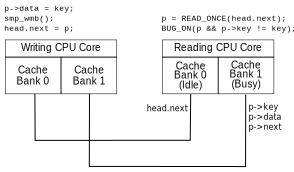
\includegraphics{memorder/Alpha}}
\caption{Why \tco{smp_read_barrier_depends()} is Required}
\label{fig:memorder:Why smp-read-barrier-depends() is Required}
\end{figure}

One could place an \co{smp_rmb()} primitive
between the pointer fetch and dereference in order to force Alpha
to order the pointer fetch with the later dependent load.
However, this imposes unneeded overhead on systems (such as ARM
Itanium, PPC, and SPARC) that respect data dependencies on the read side.
A \co{smp_read_barrier_depends()} primitive has therefore been added to the
Linux kernel to eliminate overhead on these systems.
This primitive could be inserted in place of line~19 of
Listing~\ref{lst:memorder:Insert and Lock-Free Search},
but it is better to use the \co{rcu_dereference()} wrapper macro
as shown on lines~17 and~22 of
Listing~\ref{lst:memorder:Safe Insert and Lock-Free Search}.

It is also possible to implement a software barrier
that could be used in place of \co{smp_wmb()}, which would force
all reading CPUs to see the writing CPU's writes in order.
However, this approach was deemed by the Linux community
to impose excessive overhead
on extremely weakly ordered CPUs such as Alpha, and furthermore would
not be considered a reasonable approach by those whose systems must meet
aggressive real-time response requirements.
This software barrier could be implemented by sending inter-processor
interrupts (IPIs) to all other CPUs.
Upon receipt of such an IPI, a CPU would execute a memory-barrier
instruction, implementing a memory-barrier shootdown.
Additional logic is required to avoid deadlocks.
Of course, CPUs that respect data dependencies would define such a barrier
to simply be \co{smp_wmb()}.
Perhaps this decision should be revisited in the future as Alpha
fades off into the sunset, but as of 2017 there is a surprisingly
large number of people who run recent Linux kernels on their lovingly
preserved DEC Alpha systems.

\begin{listing}[tbp]
{ \scriptsize
\begin{verbbox}
 1  struct el *insert(long key, long data)
 2  {
 3      struct el *p;
 4      p = kmalloc(sizeof(*p), GFP_ATOMIC);
 5      spin_lock(&mutex);
 6      p->next = head.next;
 7      p->key = key;
 8      p->data = data;
 9      smp_wmb();
10      head.next = p;
11      spin_unlock(&mutex);
12  }
13
14  struct el *search(long key)
15  {
16      struct el *p;
17      p = rcu_dereference(head.next);
18      while (p != &head) {
19          if (p->key == key) {
20              return (p);
21          }
22          p = rcu_dereference(p->next);
23      };
24      return (NULL);
25  }
\end{verbbox}
}
\centering
\theverbbox
\caption{Safe Insert and Lock-Free Search}
\label{lst:memorder:Safe Insert and Lock-Free Search}
\end{listing}

The Linux memory-barrier primitives took their names from the Alpha
instructions, so \co{smp_mb()} is {\tt mb}, \co{smp_rmb()} is {\tt rmb},
and \co{smp_wmb()} is {\tt wmb}.
Alpha is the only CPU where \co{smp_read_barrier_depends()} is
an \co{smp_mb()} rather than a no-op.

\QuickQuiz{}
	Why is Alpha's \co{smp_read_barrier_depends()} an
	\co{smp_mb()} rather than \co{smp_rmb()}?
\QuickQuizAnswer{
	First, Alpha has only \co{mb} and \co{wmb} instructions,
	so \co{smp_rmb()} would be implemented by the Alpha \co{mb}
	instruction in either case.

	More importantly, \co{smp_read_barrier_depends()} must
	order subsequent stores.
	For example, consider the following code:

\vspace{5pt}
\begin{minipage}[t]{\columnwidth}
\small
\begin{verbatim}
  1 p = global_pointer;
  2 smp_read_barrier_depends();
  3 if (do_something_with(p->a, p->b) == 0)
  4   p->hey_look = 1;
\end{verbatim}
\end{minipage}
\vspace{5pt}

	Here the store to \co{p->hey_look} must be ordered,
	not just the loads from \co{p->a} and \co{p->b}.
} \QuickQuizEnd

For more on Alpha, see its reference manual~\cite{ALPHA2002}.

\subsection{ARMv7-A/R}
\label{sec:memorder:ARMv7-A/R}

The ARM family of CPUs is extremely popular in embedded applications,
particularly for power-constrained applications such as cellphones.
Its memory model is similar to that of Power
(see Section~\ref{sec:memorder:POWER / PowerPC}, but ARM uses a
different set of memory-barrier instructions~\cite{ARMv7A:2010}:

\begin{description}
\item	[\tco{DMB}] (data memory barrier) causes the specified type of
	operations to \emph{appear} to have completed before any
	subsequent operations of the same type.
	The ``type'' of operations can be all operations or can be
	restricted to only writes (similar to the Alpha \co{wmb}
	and the POWER \co{eieio} instructions).
	In addition, ARM allows cache coherence to have one of three
	scopes: single processor, a subset of the processors
	(``inner'') and global (``outer'').
\item	[\tco{DSB}] (data synchronization barrier) causes the specified
	type of operations to actually complete before any subsequent
	operations (of any type) are executed.
	The ``type'' of operations is the same as that of \co{DMB}.
	The \co{DSB} instruction was called \co{DWB} (drain write buffer
	or data write barrier, your choice) in early versions of the
	ARM architecture.
\item	[\tco{ISB}] (instruction synchronization barrier) flushes the CPU
	pipeline, so that all instructions following the \co{ISB}
	are fetched only after the \co{ISB} completes.
	For example, if you are writing a self-modifying program
	(such as a JIT), you should execute an \co{ISB} between
	generating the code and executing it.
\end{description}

None of these instructions exactly match the semantics of Linux's
\co{rmb()} primitive, which must therefore be implemented as a full
\co{DMB}.
The \co{DMB} and \co{DSB} instructions have a recursive definition
of accesses ordered before and after the barrier, which has an effect
similar to that of POWER's cumulativity.

ARM also implements control dependencies, so that if a conditional
branch depends on a load, then any store executed after that conditional
branch will be ordered after the load.
However, loads following the conditional branch will \emph{not}
be guaranteed to be ordered unless there is an \co{ISB}
instruction between the branch and the load.
Consider the following example:

\vspace{5pt}
\begin{minipage}[t]{\columnwidth}
\small
\begin{verbatim}
  1 r1 = x;
  2 if (r1 == 0)
  3   nop();
  4 y = 1;
  5 r2 = z;
  6 ISB();
  7 r3 = z;
\end{verbatim}
\end{minipage}
\vspace{5pt}

In this example, load-store control dependency ordering causes
the load from \co{x} on line~1 to be ordered before the store to
\co{y} on line~4.
However, ARM does not respect load-load control dependencies, so that
the load on line~1 might well happen \emph{after} the
load on line~5.
On the other hand, the combination of the conditional branch on line~2
and the \co{ISB} instruction on line~6 ensures that
the load on line~7 happens after the load on line~1.
Note that inserting an additional \co{ISB} instruction somewhere between
lines~3 and 4 would enforce ordering between lines~1 and 5.

\subsection{ARMv8}

\begin{figure}[tb]
\centering
\resizebox{2in}{!}{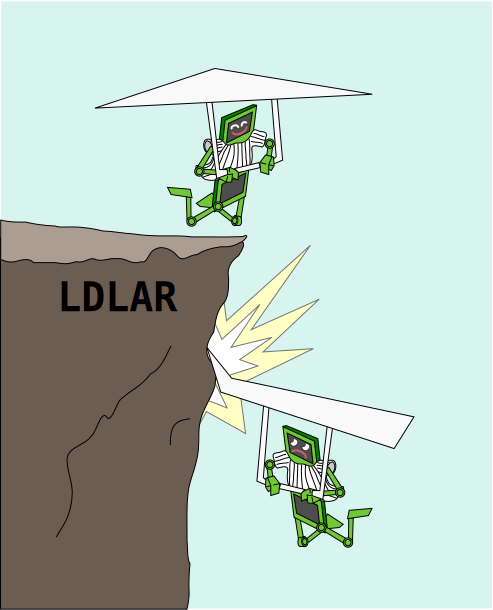
\includegraphics{cartoons/r-2014-LDLAR}}
\caption{Half Memory Barrier}
\ContributedBy{Figure}{fig:memorder:Half Memory Barrier}{Melissa Brossard}
\end{figure}

ARMv8 is ARM's 64-bit CPU~\cite{ARMv8A:2017},
in contrast to their 32-bit CPU described in
Section~\ref{sec:memorder:ARMv7-A/R}.
ARMv8's memory model closely resembles its 32-bit counterpart,
but adds load-acquire (\co{LDLARB}, \co{LDLARH}, and \co{LDLAR})
and store-release (\co{STLLRB}, \co{STLLRH}, and \co{STLLR})
instructions.
These instructions act as ``half memory barriers'', so that
ARMv8 CPUs can reorder previous accesses with a later \co{LDLAR}
instruction, but are prohibited from reordering an earlier \co{LDAR}
instruction with later accesses, as fancifully depicted in
Figure~\ref{fig:memorder:Half Memory Barrier}.
Similarly, ARMv8 CPUs can reorder an earlier \co{STLLR} instruction with
a subsequent access, but are prohibited from reordering
previous accesses with a later \co{STLLR} instruction.
As one might expect, this means that these instructions directly support
the C11 notion of load-acquire and store-release.

However, ARMv8 goes well beyond the C11 memory model by mandating that
the combination of a store-release and load-acquire act as a full
barrier under many circumstances.
For example, in ARMv8, given a store followed by a store-release followed
a load-acquire followed by a load, all to different variable, all CPUs
would agree that the initial store preceded the final load.
Interestingly enough, most TSO architectures (including x86 and the
mainframe) do not make this guarantee, as the two loads could be
reordered before the two stores.

ARMv8 also has the distinction of being the first CPU whose vendor publicly
defined its memory ordering with a formal model~\cite{ARMv8A:2017}.

\subsection{Itanium}

Itanium offers a weak consistency model, so that in absence of explicit
memory-barrier instructions, Itanium is within its rights to arbitrarily
reorder memory references~\cite{IntelItanium02v2}.
Itanium has a memory-fence instruction named {\tt mf}, but also has
``half-memory fence'' modifiers to loads, stores, and to some of its atomic
instructions~\cite{IntelItanium02v3}.
The {\tt acq} modifier prevents subsequent memory-reference instructions
from being reordered before the {\tt acq}, but permits
prior memory-reference instructions to be reordered after the {\tt acq},
similar to the ARMv8 load-acquire instructions.
Similarly, the {\tt rel} modifier prevents prior memory-reference
instructions from being reordered after the {\tt rel}, but allows
subsequent memory-reference instructions to be reordered before
the {\tt rel}.

These half-memory fences are useful for critical sections, since
it is safe to push operations into a critical section, but can be
fatal to allow them to bleed out.
However, as one of the only CPUs with this property,\footnote{
	ARMv8 has recently added load-acquire and store-release instructions.}
Itanium defines
Linux's semantics of memory ordering associated with lock acquisition
and release.
Oddly enough, actual Itanium hardware is rumored to implement
both load-acquire and store-release instructions as full barriers.
Nevertheless, Itanium was the first mainstream CPU to introduce the concept
(if not the reality) of load-acquire and store-release into its
instruction set.

The Itanium {\tt mf} instruction is used for the \co{smp_rmb()},
\co{smp_mb()}, and \co{smp_wmb()} primitives in the Linux kernel.
Oh, and despite rumors to the contrary, the ``mf'' mnemonic really
does stand for ``memory fence''.

Finally, Itanium offers a global total order for ``release'' operations,
including the ``mf'' instruction.
This provides the notion of transitivity, where if a given code fragment
sees a given access as having happened, any later code fragment will
also see that earlier access as having happened.
Assuming, that is, that all the code fragments involved correctly use
memory barriers.

\subsection{MIPS}

The MIPS memory model~\cite[Table 6.6]{MIPSvII-A-2015}
appears to resemble that of ARM, Itanium, and Power,
being weakly ordered by default, but respecting dependencies.
MIPS has a wide variety of memory-barrier instructions, but ties them
not to hardware considerations, but rather to the use cases provided
by the Linux kernel and the C++11 standard~\cite{RichardSmith2015N4527}
in a manner similar to the ARM64 additions:

\begin{description}[style=nextline]
\item[\tco{SYNC}]
	Full barrier for a number of hardware operations in addition
	to memory references.
\item[\tco{SYNC_WMB}]
	Write memory barrier, which can be used to implement the
	\co{smp_wmb()} primitive in the Linux kernel.
\item[\tco{SYNC_MB}]
	Full memory barrier, but only for memory operations.
	This may be used to implement the Linux-kernel \co{smp_mb()}
	and the C++ \co{atomic_thread_fence(memory_order_seq_cst)}.
\item[\tco{SYNC_ACQUIRE}]
	Acquire memory barrier, which may be used to implement the
	Linux-kernel \co{smp_load_acquire()} and the C++
	\co{atomic_load_explicit(..., memory_order_acquire)}.
\item[\tco{SYNC_RELEASE}]
	Release memory barrier, which may be used to implement the
	Linux-kernel \co{smp_store_release()} and the C++
	\co{atomic_store_explicit(..., memory_order_release)}.
\item[\tco{SYNC_RMB}]
	Read memory barrier, which can be used to implement the
	\co{smp_rmb()} primitive in the Linux kernel.
\end{description}

Informal discussions with MIPS architects indicates that MIPS has a
definition of transitivity or cumulativity similar to that of
ARM and Power.
However, it appears that different MIPS implementations can have
different memory-ordering properties, so it is important to consult
the documentation for the specific MIPS implementation you are using.

\subsection{PA-RISC}

Although the PA-RISC architecture permits full reordering of loads and
stores, actual CPUs run fully ordered~\cite{GerryKane96a}.
This means that the Linux kernel's memory-ordering primitives generate
no code, however, they do use the gcc {\tt memory} attribute to disable
compiler optimizations that would reorder code across the memory
barrier.

\subsection{POWER / PowerPC}
\label{sec:memorder:POWER / PowerPC}

The POWER and PowerPC\textsuperscript{\textregistered}
CPU families have a wide variety of memory-barrier
instructions~\cite{PowerPC94,MichaelLyons05a}:
\begin{description}
\item	[\tco{sync}] causes all preceding operations to {\em appear to have}
	completed before any subsequent operations are started.
	This instruction is therefore quite expensive.
\item	[\tco{lwsync}] (light-weight sync) orders loads with respect to
	subsequent loads and stores, and also orders stores.
	However, it does {\em not} order stores with respect to subsequent
	loads.
	Interestingly enough, the {\tt lwsync} instruction enforces
	the same ordering as does zSeries, and coincidentally,
	SPARC TSO.
	The \co{lwsync} instruction may be used to implement
	load-acquire and store-release operations.
\item	[\tco{eieio}] (enforce in-order execution of I/O, in case you
	were wondering) causes all preceding cacheable stores to appear
	to have completed before all subsequent stores.
	However, stores to cacheable memory are ordered separately from
	stores to non-cacheable memory, which means that {\tt eieio}
	will not force an MMIO store to precede a spinlock release.
\item	[\tco{isync}] forces all preceding instructions to appear to have
	completed before any subsequent instructions start execution.
	This means that the preceding instructions must have progressed
	far enough that any traps they might generate have either happened
	or are guaranteed not to happen, and that any side-effects of
	these instructions (for example, page-table changes) are seen by the
	subsequent instructions.
\end{description}

Unfortunately, none of these instructions line up exactly with Linux's
{\tt wmb()} primitive, which requires {\em all} stores to be ordered,
but does not require the other high-overhead actions of the {\tt sync}
instruction.
But there is no choice: ppc64 versions of {\tt wmb()} and {\tt mb()} are
defined to be the heavyweight {\tt sync} instruction.
However, Linux's \co{smp_wmb()} instruction is never used for MMIO
(since a driver must carefully order MMIOs in UP as well as
SMP kernels, after all), so it is defined to be the lighter weight
{\tt eieio} instruction.
This instruction may well be unique in having a five-vowel mnemonic.
The \co{smp_mb()} instruction is also defined to be the {\tt sync}
instruction, but both \co{smp_rmb()} and \co{rmb()} are defined to
be the lighter-weight {\tt lwsync} instruction.

Power features ``cumulativity'', which can be used to obtain
transitivity.
When used properly, any code seeing the results of an earlier
code fragment will also see the accesses that this earlier code
fragment itself saw.
Much more detail is available from
McKenney and Silvera~\cite{PaulEMcKenneyN2745r2009}.

Power respects control dependencies in much the same way that ARM
does, with the exception that the Power \co{isync} instruction
is substituted for the ARM \co{ISB} instruction.

Many members of the POWER architecture have incoherent instruction
caches, so that a store to memory will not necessarily be reflected
in the instruction cache.
Thankfully, few people write self-modifying code these days, but JITs
and compilers do it all the time.
Furthermore, recompiling a recently run program looks just like
self-modifying code from the CPU's viewpoint.
The {\tt icbi} instruction (instruction cache block invalidate)
invalidates a specified cache line from
the instruction cache, and may be used in these situations.

\subsection{SPARC RMO, PSO, and TSO}

Solaris on SPARC uses TSO (total-store order), as does Linux when built for
the ``sparc'' 32-bit architecture.
However, a 64-bit Linux kernel (the ``sparc64'' architecture)
runs SPARC in RMO (relaxed-memory order) mode~\cite{SPARC94}.
The SPARC architecture also offers an intermediate PSO (partial store
order).
Any program that runs in RMO will also run in either PSO or TSO, and similarly,
a program that runs in PSO will also run in TSO.
Moving a shared-memory parallel program in the other direction may
require careful insertion of memory barriers, although, as noted earlier,
programs that make standard use of synchronization primitives need not
worry about memory barriers.

SPARC has a very flexible memory-barrier instruction~\cite{SPARC94}
that permits fine-grained control of ordering:
\begin{description}
\item	[\tco{StoreStore}] orders preceding stores before subsequent stores.
	(This option is used by the Linux \co{smp_wmb()} primitive.)
\item	[\tco{LoadStore}] orders preceding loads before subsequent stores.
\item	[\tco{StoreLoad}] orders preceding stores before subsequent loads.
\item	[\tco{LoadLoad}] orders preceding loads before subsequent loads.
	(This option is used by the Linux \co{smp_rmb()} primitive.)
\item	[\tco{Sync}] fully completes all preceding operations before starting
	any subsequent operations.
\item	[\tco{MemIssue}] completes preceding memory operations before subsequent
	memory operations, important for some instances of memory-mapped
	I/O.
\item	[\tco{Lookaside}] does the same as MemIssue,
	but only applies to preceding stores
	and subsequent loads, and even then only for stores and loads that
	access the same memory location.
\end{description}

The Linux \co{smp_mb()} primitive uses the first four options together,
as in
\co{membar #LoadLoad | #LoadStore | #StoreStore | #StoreLoad},
thus fully ordering memory operations.

So, why is \qco{membar #MemIssue} needed?
Because a \qco{membar #StoreLoad} could permit a subsequent
load to get its value from a store buffer, which would be
disastrous if the write was to an MMIO register that induced side effects
on the value to be read.
In contrast, \qco{membar #MemIssue} would wait until the store buffers
were flushed before permitting the loads to execute,
thereby ensuring that the load actually gets its value from the MMIO register.
Drivers could instead use \qco{membar #Sync}, but the lighter-weight
\qco{membar #MemIssue} is preferred in cases where the additional function
of the more-expensive \qco{membar #Sync} are not required.

The \qco{membar #Lookaside} is a lighter-weight version of
\qco{membar #MemIssue}, which is useful when writing to a given MMIO register
affects the value that will next be read from that register.
However, the heavier-weight \qco{membar #MemIssue} must be used when
a write to a given MMIO register affects the value that will next be
read from {\em some other} MMIO register.

It is not clear why SPARC does not define \co{wmb()} to be
\qco{membar #MemIssue} and \co{smp_wmb()} to be
\qco{membar #StoreStore},
as the current definitions seem vulnerable to bugs in some drivers.
It is quite possible that all the SPARC CPUs that Linux runs on
implement a more conservative memory-ordering model than the architecture
would permit.

SPARC requires a {\tt flush} instruction be used between the time that
an instruction is stored and executed~\cite{SPARC94}.
This is needed to flush any prior value for that location from
the SPARC's instruction cache.
Note that {\tt flush} takes an address, and will flush only that address
from the instruction cache.
On SMP systems, all CPUs' caches are flushed, but there is no
convenient way to determine when the off-CPU flushes complete,
though there is a reference to an implementation note.

\subsection{x86}

Since the x86 CPUs provide ``process ordering'' so that all CPUs agree
on the order of a given CPU's writes to memory, the \co{smp_wmb()} primitive
is a no-op for the CPU~\cite{IntelXeonV3-96a}.
However, a compiler directive is required to
prevent the compiler from performing optimizations that would result
in reordering across the \co{smp_wmb()} primitive.

On the other hand, x86 CPUs have traditionally given
no ordering guarantees for loads, so
the \co{smp_mb()} and \co{smp_rmb()} primitives expand to {\tt lock;addl}.
This atomic instruction acts as a barrier to both loads and stores.

Intel has also published a memory model for
x86~\cite{Intelx86MemoryOrdering2007}.
It turns out that Intel's actual CPUs enforced tighter ordering than
was claimed in the previous specifications, so this model is in effect
simply mandating the earlier de-facto behavior.
Even more recently, Intel published an updated memory model for
x86~\cite[Section 8.2]{Intel64IA32v3A2011}, which mandates a total global order
for stores, although individual CPUs are still permitted to see their
own stores as having happened earlier than this total global order
would indicate.
This exception to the total ordering is needed to allow important
hardware optimizations involving store buffers.
In addition, memory ordering obeys causality, so that if CPU~0 sees a
store by CPU~1, then CPU~0 is guaranteed to see all stores that CPU~1
saw prior to its store.
Software may use atomic operations to override these hardware optimizations,
which is one reason that atomic operations tend to be more expensive
than their non-atomic counterparts.
This total store order is \emph{not} guaranteed on older processors.

It is also important to note that atomic instructions operating
on a given memory location should all be of the same
size~\cite[Section 8.1.2.2]{Intel64IA32v3A2011}.
For example, if you write a program where one CPU atomically increments
a byte while another CPU executes a 4-byte atomic increment on
that same location, you are on your own.

However, note that some SSE instructions are weakly ordered ({\tt clflush}
and non-temporal move instructions~\cite{IntelXeonV2b-96a}).
CPUs that have SSE can use {\tt mfence} for \co{smp_mb()},
{\tt lfence} for \co{smp_rmb()}, and {\tt sfence} for \co{smp_wmb()}.

A few versions of the x86 CPU have a mode bit that enables out-of-order
stores, and for these CPUs, \co{smp_wmb()} must also be defined to
be {\tt lock;addl}.

Although newer x86 implementations accommodate self-modifying code
without any special instructions, to be fully compatible with
past and potential future x86 implementations, a given CPU must
execute a jump instruction or a serializing instruction (e.g., \co{cpuid})
between modifying the code and executing
it~\cite[Section 8.1.3]{Intel64IA32v3A2011}.

\subsection{zSeries}

The zSeries machines make up the IBM\textsuperscript{\texttrademark}
mainframe family, previously
known as the 360, 370, and 390~\cite{IBMzSeries04a}.
Parallelism came late to zSeries, but given that these mainframes first
shipped in the mid 1960s, this is not saying much.
The \qco{bcr 15,0} instruction is used for the Linux \co{smp_mb()},
\co{smp_rmb()}, and \co{smp_wmb()} primitives.
It also has comparatively strong memory-ordering semantics, as shown in
Table~\ref{tab:memorder:Summary of Memory Ordering}, which should allow the
\co{smp_wmb()} primitive to be a {\tt nop} (and by the time you read this,
this change may well have happened).
The table actually understates the situation, as the zSeries memory model
is otherwise sequentially consistent, meaning that all CPUs
will agree on the order of unrelated stores from different CPUs.

As with most CPUs, the zSeries architecture does not guarantee a
cache-coherent instruction stream, hence,
self-modifying code must execute a serializing instruction between updating
the instructions and executing them.
That said, many actual zSeries machines do in fact accommodate self-modifying
code without serializing instructions.
The zSeries instruction set provides a large set of serializing instructions,
including compare-and-swap, some types of branches (for example, the
aforementioned \qco{bcr 15,0} instruction), and test-and-set,
among others.

\section{Where is Memory Ordering Needed?}
\label{sec:memorder:Where is Memory Ordering Needed?}

This section revisits
Table~\ref{tab:memorder:Linux-Kernel Memory-Ordering Cheat Sheet}
in light of the intervening discussion.

Memory-ordering operations are only required where there is a possibility
of interaction involving at least two variables between at least two
threads.
As always, if a single-threaded program will provide sufficient
performance, why bother with parallelism?\footnote{
	Hobbyists and researchers should of course feel free to ignore
	this and other cautions.}
After all, avoiding parallelism also avoids the added cost of
memory-ordering operations.

If all thread-to-thread communication in a given cycle use store-to-load links
(that is, the next thread's load returning the value that the previous thread
stored), minimal ordering suffices.
Minimal ordering includes dependencies, acquires, and all stronger
ordering operations.

If all but one of the links in a given cycle is a store-to-load
link, it is sufficient to use release-acquire pairs for each of
those store-to-load links.
You can replace a given acquire with a a dependency in environments permitting
this, keeping in mind that the C11 standard's memory model does \emph{not}
permit this.
Note also that a dependency leading to a load must be headed by
a \co{lockless_dereference()} or an \co{rcu_dereference()}:
\co{READ_ONCE()} is not sufficient.
Never forget to carefully review
Sections~\ref{sec:memorder:Address- and Data-Dependency Restrictions}
and~\ref{sec:memorder:Control-Dependency Restrictions}, because
a dependency broken by your compiler is no help at all!
The two threads sharing the sole non-store-to-load link can
usually substitute \co{WRITE_ONCE()} plus \co{smp_wmb()} for
\co{smp_store_release()} on the one hand,
and \co{READ_ONCE()} plus \co{smp_rmb()} for \co{smp_load_acquire()}
on the other.

If a given cycle contains two or more non-store-to-load links (that is,
a total of two or more load-to-store and store-to-store links), you will
need at least one strong barrier between each pair of non-store-to-load
links in that cycle.
Strong barriers include \co{smp_mb()}, successful full-strength non-\co{void}
atomic RMW operations, and other atomic RMW operations in conjunction with
either \co{smp_mb__before_atomic()} or \co{smp_mb__after_atomic()}.
With strength comes expense, though the overhead of strong barriers
usually hurts performance more than it hurts scalability.

Note that these are the \emph{minimum} guarantees.
Different architectures may give
more substantial guarantees,
as discussed in Section~\ref{sec:memorder:Hardware Specifics},
but they may \emph{not}
be relied upon outside of code specifically designed to run only on
the corresponding architecture.

One final word of advice: Again, use of raw memory-ordering primitives is
a last resort.
It is almost always better to use existing primitives, such as locking
or RCU, that take care of memory ordering for you.
